% !TEX root = phy315book.tex


%----------------------------------------------------------------------------------------
%	PART 2 12-22
%----------------------------------------------------------------------------------------
\part{Using Quantum States \label{part2}}

We now move on to using quantum states model a number of different systems.

\begin{figure}
\centering
\begin{tikzpicture}
\node[fill=blue!20,arrow box, text width=4.5cm, align=center, arrow box arrows={south:1cm},arrow box shaft width=1cm](p1) at (0,10) {\Large Time Evolution of Quantum States};
\node[fill=blue!20,arrow box, text width=4.5cm, align=center, arrow box arrows={south:1cm},arrow box shaft width=1cm](p2) at (0,8) {\Large Uncertainty in Measurement};
\node[fill=blue!20,arrow box, text width=4.5cm, align=center, arrow box arrows={south:1cm},arrow box shaft width=1cm](p3) at (0,6) {\Large Entanglement};
\node[fill=blue!20,rectangle, text width=4.5cm, align=center](p4) at (0,4) {\Large Continuous Eigenvalues};
\node[fill=blue!20,rectangle, text width=4.5cm, align=center](p4) at (0,2) {\Large Matter Wave Models};

\end{tikzpicture}
\end{figure}


\chapter{Time Evolution of a Quantum State}
Ok, we've got tools to model two types of quantum systems using our state vectors and linear operators. But at this point, we've only described a static system. How does a quantum state evolve in time? Another way of looking at this is: how does the quantum state change due to interactions with other things? We've already seen examples of interactions: the \hwp and \qwp somehow change the quantum state. There is an equivalent interaction for the quantum spin: a {\em uniform} magnetic field.

\marginnote{This is the same idea as the kinematics equation for a point particle: $x(t)=x(0) + \dot{x}(0)t + (1/2) a t^2$. Give me an initial position and velocity and tell me the interaction ($a$) and I can tell you how the particle moves.}So what we want is a model that takes our quantum state at time $t=0$ and gives us the state at some future time $t$:
\beq
\ket{\Psi(t)} = \hat{U}(t)\ket{\Psi(0)}.
\label{eq:unittime}
\eeq
where $\hat{U}(t)$ is some operator that tells us how the interactions change the quantum state. There is a conceptual point here that I need to make: What this model is saying is that the time evolution of the quantum state is {\em predictable}. Our model predicts what the quantum state will be. However, our measurement outcomes will still be {\em probabilistic}. 

\section{Properties of $\hat{U}$}

What can we say about this evolution operator $\hat{U}$? Well, to start, we'd like it to not change the normalization properties of quantum states. Say we have a quantum state that, at time $t=0$, is normalized:
\beq
\avg{\Psi(0)|\Psi(0)}=1,
\eeq
then we want these states to remain normalized at any future time:
\beq
\avg{\Psi(t)|\Psi(t)}=1.
\eeq
We re-write this in terms of $\hat{U}$ (and use the bra vector version of Eq.~(\ref{eq:unittime}) $\bra{\Psi(t)} = \bra{\Psi(0)}\hat{U}^\dagger(t)$). This means that
\beq
\avg{\Psi(t)|\Psi(t)}=\bra{\Psi(0)} \underbrace{\hat{U}^\dagger(t) \hat{U}(t)}_{\rmt{This must be } 1}\ket{\Psi(0)} = 1.
\eeq
So the combination of $\hat{U}^\dagger(t) \hat{U}(t)$ must be some ``one'' operator that doesn't change the states. We'll denote this as $\onehat$ such that
\beq
\onehat \ket{\Psi} = \ket{\Psi}.
\eeq
Using this notation, we get $\hat{U}^\dagger(t) \hat{U}(t) = \onehat$. If we move the $\hat{U}$ to the other side we have that the Hermitian conjugate is equal to the inverse of $\hat{U}$,
\beq
\hat{U}^\dagger(t) = \hat{U}^{-1}(t).
\eeq
This is the definition of a {\em unitary operator}. This type of operator doesn't change the normalization of a state vector. \arnote{Your turn: follow the same reasoning to show that a unitary operator also maintains orthogonality between two orthogonal state vectors.}


\section{Small Time Steps}
\label{sec:scheqn}
If our unitary time evolution operator works for some time $t$, then it should also work for some very short time $\epsilon$. But we should also find that our quantum state hasn't changed very much in that small time step. So, applying what we know from above, that means that $\hat{U}^\dagger(\epsilon) \hat{U}(\epsilon) = \onehat$. We now write our unitary operator as a small linear step away from the $\onehat$ operator since we are taking only a very small time step:\marginnote{The units of $\epsilon/\hbar$ are s$^{2}$/(kg m$^2$) = 1/J, so $\hat{H}$ must have units of energy.}
\beq
\hat{U}(\epsilon) = \onehat -\frac{\I\epsilon}{\hbar} \hat{H}
\eeq
where we've written the small time evolution in terms of a Hermitian operator $\hat{H}$ which we call the {\em Hamiltonian}. We will show later that this operator models the total energy of a system. The Hermitian conjugate of $\hat{U}(\epsilon)$ is
\beq
\hat{U}^\dagger(\epsilon) = \onehat +\frac{\I\epsilon}{\hbar} \hat{H}.
\eeq
Now we write the quantum state at time step $\epsilon$ using this linear approximation:
\beq
\ket{\Psi(\epsilon)} = \ket{\Psi(0)} - \frac{\I\epsilon}{\hbar} \hat{H} \ket{\Psi(0)}.
\eeq
We rearrange this to get
\beq
\frac{\ket{\Psi(\epsilon)} - \ket{\Psi(0)}}{\epsilon}  = - \frac{\I}{\hbar} \hat{H} \ket{\Psi(0)}.
\eeq
\marginnote{This is equivalent in importance to our quantum model as Newton's 2nd Law, $\vec{F}=m (d^2\vec{x}/dt^2)$, is to classical mechanics.}
But the piece on the left-hand side is just the definition of a time derivative in the limit where $\epsilon\rightarrow 0$. So we have, finally, the {\em Schr\"{o}dinger equation}:\toolnote[0.2cm]{\toollabel{tool:sch}{\includegraphics{tool7.tikz} {\bf Schr\"{o}dinger Equationator}}  This tool is used to find the time evolution of a quantum state.} 
\beq
\I \hbar \frac {d}{dt}\ket{\Psi} = \hat{H}\ket{\Psi}
\label{eq:sch}
\eeq
which is the fundamental equation of ``motion'' or time evolution for our quantum model.

\section{Time-Independent Schr\"{o}dinger Equation}
We will encounter many situations where the Hamiltonian operator does not depend explicitly on time, or 
\beq
\frac{d\hat{H}}{dt}=0.
\eeq
This is very similar to the model from classical mechanics that the total mechanical energy is conserved. In that model, we found the total energy of the system and then used that to make predictions about the time evolution of the system. The same type of model works here: we find the eigenvectors and eigenvalues of the Hamiltonian operator and then we use this to make predictions about the time evolution of the system. Although the first part is the hard part (we'll spend a lot of time on it later), we'll assume for now that we've got it done. We call the eigenvectors $\ket{E}$ with corresponding eigenvalues $E$:
\beq
\hat{H}\ket{E} = E\ket{E}. 
\eeq\marginnote[-1cm]{\ref{tool:eigen}}%
Following our Technique \ref{tec:expec}, we expand our quantum state in terms of these eigenvalues,
\beq
\ket{\Psi(t)} = \sum_E a_E(t)\ket{E}, 
\eeq\marginnote[-1cm]{\ref{tool:decom}}%
where we are using $a_E(t)$ to represent the expansion coefficients $\alpha_j$. Since the total energy of the system doesn't change with time, the eigenvectors $\ket{E}$ also don't change. So all of the evolution of the quantum state has to be in the coefficients.

We now use this expansion with the Schr\"{o}dinger equation (Eq.~(\ref{eq:sch})) to determine how the coefficients $a_E(t)$ evolve with time.
\marginnote[2.5cm]{\ref{tool:decom}}%
\bas
\I \hbar \frac {d}{dt}\ket{\Psi(t)} & = \hat{H}\ket{\Psi(t)} \\
\downarrow \phantom{spa} & \phantom{spa} \downarrow \nonumber\\
\I\hbar\frac{d}{dt}\left[\sum_E a_E(t)\ket{E} \right] & =  \hat{H}\left[\sum_E a_E(t)\ket{E} \right]  \\
\downarrow \phantom{spa} & \phantom{spa} \downarrow \nonumber\\
\I\hbar\sum_E \frac{d a_E(t)}{dt}\ket{E} & =  \sum_E a_E(t)\hat{H}\ket{E} \\
{} &= \sum_E a_E(t)E\ket{E}.
\eas\marginnote[-1.9cm]{\ref{tool:eigen}}
So, we have, putting everything on the same side,
\beq
\sum_E \left[ \I\hbar\frac{d a_E(t)}{dt} - Ea_E(t)\right]\ket{E} = 0.
\eeq
The only way this works is if every term in the square brackets is zero. This means that
\beq
\I\hbar\frac{d a_E(t)}{dt} = Ea_E(t).
\eeq
The solution to this is:\arnote{Check this if you haven't solved differential equations in awhile.}
\beq
a_E(t) = a_E(0)\E{-\I Et/\hbar},
\eeq
where $a_E(0)$ is a constant: the value of $a_E$ when $t=0$. 
So, the solution to the Schr\"{o}dinger equation, when the Hamiltonian is time-independent, is
\beq
\ket{\Psi(t)} = \sum_E a_E(0)\E{-\I Et/\hbar}\ket{E}.
\label{eq:soltoTDSE}
\eeq

\begin{tacticsbox}
\label{tactis:TISE}
To solve the time-independent Schr\"{o}dinger equation:
\begin{enumerate}
\item Model the interaction as a time-independent Hamiltonian (based on the total energy of the system) as an operator $\hat{H}$.
\item Find the eigenvalues $E$ and eigenvectors $\ket{E}$ of the Hamiltonian $\hat{H}$:
\beq
\hat{H}\ket{E} = E\ket{E}
\eeq
\item Model the system as a quantum state at the inital time $t=0$ and expand the quantum state in terms of the Hamiltonian eigenvectors:
\beq
\ket{\Psi(0)} = \sum_E a_E(0)\ket{E}.
\eeq
where $a_E(0) = \avg{E|\Psi(0)}$.
\item Write down the evolution of the quantum state inserting $\E{-\I Et/\hbar}$:
\beq
\ket{\Psi(t)} = \sum_E a_E(0)\E{-\I Et/\hbar} \ket{E}.
\eeq
\end{enumerate}
\end{tacticsbox}
\marginnote[-1.4cm]{Using \ref{tool:orthog}}%
Now we'll do some practicing and some examples.
\begin{exercise}
Suppose at $t = 0$ an atom is in the state 
\beq
\ket{\Psi(0)} = \frac{1}{2}\ket{E_1} + \I\frac{\sqrt{3}}{2}\ket{E_2},
\eeq
%
where $\ket{E_1}$ and $\ket{E_2}$ are two energy eigenstates of the system Hamiltonian
$\hat{H}$.

\begin{enumerate}

\item[(a)]  What is $\ket{\Psi(t)} $ for $t > 0$?

\item[(b)]  If the energy is measured at $t >  0$, find the probability of obtaining $E_{2}$.  Does this probability depend on time?
\end{enumerate}
\end{exercise}

We now run through an example to get a feel for what this means and how it works for a physical system.
\begin{example}
An atomic spin oriented in the $+x$-direction is directed through a region of uniform magnetic field, pointed in the $z$-direction. What is the time evolution of the spin in the magnetic field region?

\model We will model the magnetic field as having a magnitude $B$ pointed in the $\hat{z}$ direction. The total mechanical energy (ignoring the constant translational kinetic energy) of the spin in the magnetic field is 
\beq
H = -\vec{\mu}\cdot\vec{B} = -\frac{q}{2m}S_zB. 
\eeq\marginnote[-1.5cm]{Using Eq.~(\ref{eq:dipolespin})}%
So we model the interaction as an operator
\beq
\hat{H} =  -\gamma B \hat{S}_z,
\eeq
where we've put all the extra constants in the value $\gamma$ to make it easier to write. There are also the Land\'{e} factors to keep track of, too.

\vis We model the spin interaction schematically:
\begin{figure}
\centering
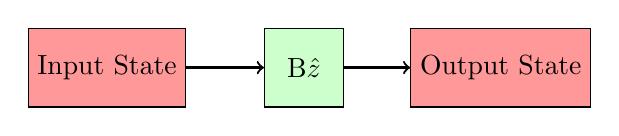
\begin{tikzpicture}
\node[fill=red!40,shape=rectangle,draw,minimum size=1cm](S) at (-0.5,0){Input State};
\node[fill=green!20,shape=rectangle,draw,minimum size=1cm](SG1) at (2,0){B$\hat{z}$};
\draw[->,thick] (S) -- (SG1);
\node[fill=red!40,shape=rectangle,draw,minimum size=1cm](S4) at (4.5,0){Output State};
\draw[->,thick] (SG1) -- (S4);
\end{tikzpicture}
\end{figure}

\sol We already know the eigenvalues and eigenvectors of our Hamiltonian. They are:
\bas
\hat{H}\ket{u}=-\gamma B\hat{S}_z\ket{u} &= -\gamma B \frac{\hbar}{2}\ket{u} \rmt{ and}\\
\hat{H}\ket{d}=-\gamma B\hat{S}_z\ket{d} &= \gamma B \frac{\hbar}{2}\ket{d}.
\eas
So our eigenvalues are $\mp \gamma B \hbar/2$ for the $\ket{u}$ and $\ket{d}$ eigenstates.

The next step is to write the input state in terms of the eigenvectors of the Hamiltonian. Since we are given a state that starts in $+x$, that means we have
\beq
\ket{r} = \frac{1}{\stwo} \ket{u} + \frac{1}{\stwo} \ket{d} 
\eeq
and $a_{u}(0) = a_{d}(0) = 1/\stwo$. So the time evolution of the state is
\beq
\ket{\Psi(t)} = \frac{1}{\stwo}\E{\I \gamma B t/2}\ket{u} + \frac{1}{\stwo}\E{-\I \gamma B t/2}\ket{d}.
\eeq
\assess Is our state still normalized? We check that  $\avg{\Psi(t)|\Psi(t)} =1$, so we are good.\arnote{Be sure to work through this explicitly. Use $\avg{u|d}=0$ to simplify.}
\end{example}

\begin{exercise}
An atomic spin oriented in the $+x$-direction is directed through a region of uniform magnetic field, pointed in the $z$-direction. What is the time evolution of the spin in the magnetic field region in the $x$-basis? We want to know this so we can predict the outcome of a measurement in the $x$-direction.
\end{exercise}

\begin{exercise}
  At $t = 0$, a neutron is oriented in the $-y$-direction ($\ket{o}$). The neutron is placed in a uniform magnetic field $\vec{B} = 10^{-5}\hat{z}$~T. 
  
\begin{enumerate}
\item[(a)]  If the neutron is measured in the $z$-basis $1$ millisecond later, find the probability of obtaining $+\hbar/2$.
\item[(b)]  If  instead the neutron is measured in the $y$-basis $1$ millisecond from $t=0$, find the probability of obtaining $+\hbar/2$.
\end{enumerate}

\end{exercise}

\begin{exercise}
I give you a quantum system with a Hamiltonian $\hat{H}$ and an observable operator $\hat{A}$ given (in the the same basis):
\beq
\hat{H}\Meq  E_1 \begin{pmatrix}1&0&0\\ 0&2&0 \\ 0&0&3\end{pmatrix}\;\;\hat{A}\Meq  a_1 \begin{pmatrix}1&0&0\\ 0&2&0 \\ 0&0&1\end{pmatrix},
\eeq
and the system is prepared in the state
\beq
\ket{\Psi(0)} \Meq  \frac{1}{3} \begin{pmatrix}1\\0\\0\end{pmatrix} -\frac{\I}{3}\begin{pmatrix}0\\1\\0\end{pmatrix} + \frac{\sqrt{7}}{3}\begin{pmatrix}0\\0\\1\end{pmatrix}.
\eeq
\begin{enumerate}
\item[(a)]  What is $\ket{\Psi(t)}$ for $t>0$?
\item[(b)]  If $\hat{A}$ is measured at $t>0$, what are the possible results? What are the probabilities for obtaining those results? What is the state of the system after each of the possible measurements?
\item[(c)] If many measurements of $\hat{A}$ are made on identical copies of $\ket{\Psi}$, what would the average results be?
\end{enumerate}

\end{exercise}


\chapter{Commutators and Measurement Uncertainty}

\section{Commutators}
Now that we have tools for modeling the time evolution of a quantum state, we need to connect these back to our model of measurable quantities as linear operators. What happens to the average of a measurement over time? We start with a general observable $\hat{L}$. The expectation value is
\beq
\avg{\hat{L}} = \bra{\Psi(t)}\hat{L}\ket{\Psi(t)}.
\eeq
How does this change with time? Let's look at the time derivative (using the product rule from calculus):
\marginnote{Using the \ref{tool:sch} Twice.}
\bas
&\frac{d}{dt}\avg{\hat{L}}\nonumber\\
& = \underbrace{ \left[\frac{d}{dt}\bra{\Psi(t)}\right]}\hat{L}\ket{\Psi(t)} +\bra{\Psi(t)}\left(\frac{\partial}{\partial t}\hat{L}\right)\ket{\Psi(t)}+  \bra{\Psi(t)}\hat{L} \underbrace{\left[\frac{d}{dt}\ket{\Psi(t)}\right]}.\nonumber\\
& \frac{d}{dt}\bra{\Psi(t)} = \frac{\I}{\hbar}\hat{H} \phantom{\ket{\Psi(t)}+\bra{\Psi(t)}\left(\frac{d}{dt}\hat{L}\right)\ket{\Psi(t)}+}\frac{d}{dt}\ket{\Psi(t)} = -\frac{\I}{\hbar}\hat{H}
\eas

We combine the two operator terms and write the middle term as an expectation value:\marginnote{Note here that the order of the operators matters. You may have seen this in 3D rotations, or in matrix multiplication. We can't just change operator order without being careful.}
\bas
\frac{d}{dt}\avg{\hat{L}} & =  \frac{\I}{\hbar}\bra{\Psi(t)}\com{\hat{H}\hat{L}-\hat{L}\hat{H}}\ket{\Psi(t)} + \avg{\frac{\partial}{\partial t}\hat{L}}\\
{} & =  \frac{\I}{\hbar}\avg{\com{\hat{H},\hat{L}}} + \avg{\frac{\partial}{\partial t}\hat{L}}\label{eq:timeop}
\eas

We will see the combination of operators $\hat{A}\hat{B} - \hat{B}\hat{A}$ often enough that we've given it a name: the {\em commutator} and define it as\toolnote{\toollabel{tool:commutator}{\includegraphics{tool8.tikz} {\bf Commutatanator}}  This tool is used to find the commutation relationship between two operators.}
\beq
\com{\hat{A},\hat{B}}=\hat{A}\hat{B} - \hat{B}\hat{A}.
\label{eq:commutator}
\eeq
\begin{example}
How is $\com{\hat{A},\hat{B}}$ related to $\com{\hat{B},\hat{A}}$?

\model We're obviously modeling our observables as linear Hermitian operators.

\vis We could visualize this abstractly as rotations in 3D space. But that doesn't really help.

\sol If $\com{\hat{A},\hat{B}}=\hat{A}\hat{B} - \hat{B}\hat{A}$ and $\com{\hat{B},\hat{A}}=\hat{B}\hat{A} - \hat{A}\hat{B}$, then, since the operators are linear, we have that
\beq \com{\hat{A},\hat{B}} = - \com{\hat{B},\hat{A}}
\eeq

\assess The relationship makes sense: we are going backwards, so we get the negative result.

\end{example}

\begin{example}
\label{ex:spincommutator}
What is the communtator $\com{\hat{S}_z,\hat{S}_x}$?

\model We're modeling the observables as linear operators. We'll use the matrix representation from Eq.~(\ref{eq:sspins}) in the $\ket{u}$---$\ket{d}$ basis. 
\bas
\hat{S}_z &\Meq  \frac{\hbar}{2}\szmatrix \\
\hat{S}_x &\Meq  \frac{\hbar}{2}\sxmatrix 
\eas
The commutator then becomes a matrix multiplication:
\beq
\hat{S}_z\hat{S}_x \Meq  \frac{\hbar^2}{4}\szmatrix\sxmatrix = \frac{\hbar^2}{4}\begin{pmatrix}0&1\\-1&0\end{pmatrix}
\eeq
and
\beq
\hat{S}_x\hat{S}_z \Meq  \frac{\hbar^2}{4}\sxmatrix\szmatrix = \frac{\hbar^2}{4}\begin{pmatrix}0&-1\\1&0\end{pmatrix}.
\eeq
Subtracting these, we get
\beq
\com{\hat{S}_z,\hat{S}_x} \Meq  \frac{\hbar^2}{2}\begin{pmatrix}0&1\\-1&0\end{pmatrix}.
\eeq
But this is just $\I\hbar\hat{S}_y$! So it looks like the commutator has a circular relationship. \arnote{Show that this works for the other two commutation relationships.}

\assess The commutator has units $\hbar^2$ since we are multipling two spins. The result $\I\hbar\hat{S}_y$ has the same units, so we are good. We have, therefore, the relationships
\bas
\com{\hat{S}_x,\hat{S}_y} =& \I\hbar\hat{S}_z\\
\com{\hat{S}_y,\hat{S}_z} =& \I\hbar\hat{S}_x\\
\com{\hat{S}_z,\hat{S}_x} =& \I\hbar\hat{S}_y.
\eas
\end{example}
%
%
\begin{exercise}
Practice the idea of the commutator by trying the various permutations of
\bas
\com{\hat{\sigma}_1,\hat{\sigma}_2}&=?\\
\com{\hat{\sigma}_2,\hat{\sigma}_3}&=?\\
\com{\hat{\sigma}_3,\hat{\sigma}_1}&=?
\eas
\end{exercise}



\section{Conservation Laws}
Going back to Eq.~(\ref{eq:timeop}), we can set conditions under which the average value of an observable is conserved, or doesn't change with time. If
\beq
\com{\hat{H},\hat{L}} = 0 \rmt{ and } \avg{\frac{\partial}{\partial t}\hat{L}}=0
\eeq
then $\avg{\hat{L}}$ is constant. This means that the expectation value is conserved. Going back to Noether's theorem, it means that there is some type of symmetry to the situation. We will encounter many operators that are not explicitly time dependent so that 
\beq
\avg{\frac{\partial}{\partial t}\hat{L}}=0.
\eeq
It thus becomes only a matter of checking if the operator commutes with the Hamiltonian to see if the expectation value remains unchanged.

\begin{exercise}
\label{ex:timeex}
Consider a silver atom in a uniform magnetic field $\vec{B}= B\hat{z}$ with a spin pointed initially in the $+y$-direction.
\begin{enumerate}
\item[(a)] What is $\ket{\Psi(t)}$ for $t > 0$?
\item[(b)] For these atoms, for $t > 0$ what is $\avg{\hat{S}_x}$?
\item[(c)] Show Eq.~(\ref{eq:timeop}) is valid for this system for $\hat{L}=\hat{S}_x$ by separately evaluating both sides of the equation.
\item[(d)] Use Eq.~(\ref{eq:timeop}) to evaluate $d\avg{\hat{S}_z}/dt$ for this state.
\end{enumerate}
\end{exercise}

\section{Uncertainty in Measurement}
Up to this point we've talked about how our measurement model is random- we can't predict the outcome of any specific measurement, though we can predict what the average of many identical measurements will be. This system is similar to the Gaussian probability distribution function that we've used many times in making statistical measurements of physical quantities. Once we have an average measurement, the next question is: what is the uncertainty in that measurement? We will use the definition of the standard deviation from statistics:
\beq
\sigma_x = \left[\sum_{i=1}^{N}(x_i - \bar{x})^2\right]^{1/2}
\eeq
where $\bar{x}$ is the average of the measurements. In terms of our quantum model, the uncertainty in the measurement of an observable $\hat{L}$ of quantum state $\ket{\Psi}$ is defined as
\beq
\Delta L \equiv \left[\bra{\Psi}(\hat{L} - \avg{\hat{L}})^2\ket{\Psi}\right]^{1/2}.
\label{eq:uncert}
\eeq
We will often re-write this in terms of the averages of both $\hat{L}$ and $\hat{L}^2$:\arnote[-1cm]{Expand Eq.~(\ref{eq:uncert}) and combine terms to get here. Note that I've squared both sides to simplify writing it. Also note that $\avg{\hat{L}^2} = \bra{\Psi}(\hat{L}\hat{L})\ket{\Psi}$.}
\beq
\Delta L^2 = \avg{\hat{L}^2} - \avg{\hat{L}}^2.
\eeq
We take the square root of both sides to get the uncertainty in the measurement of the operator $\hat{L}$:\toolnote{\toollabel{tool:meunc}{\includegraphics{tool9.tikz} {\bf Uncertainty Evaluator}}  This tool is used to find the uncertainty in the measurement associated with an operator.}
\beq
\Delta L= \left[\avg{\hat{L}^2} - \avg{\hat{L}}^2\right]^{1/2}.
\label{eq:meunc}
\eeq
The uncertainty in the measurement tells us about the range of possible measurements of our quantum state. 

\begin{example}
\label{example:uncertd}
What is the uncertainty in measuring the polarization state $\ket{D_L}$ in the $V-H$ basis?

\model We model the quantum state as $\ket{D_L}$ which, following our Technique~\ref{tec:expec}, we need to write in our measurement basis. We'll model the measurement as the linear operator $\hat{\sigma}_3$.

\vis 

\begin{figure}
\centering
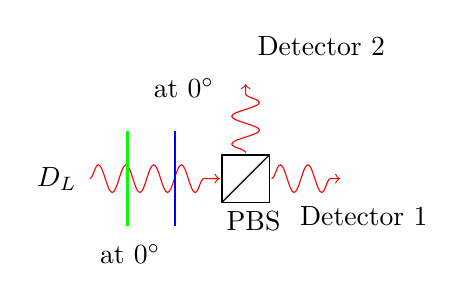
\begin{tikzpicture}[scale=0.6]
\draw (-0.5,-.5) rectangle +(1,1) node[below,shift={(-.2,-.6)}]{PBS};
\draw (-.5,-.5) -- (.5,.5);
\draw[red,->,decorate, decoration={snake,amplitude=5,segment length=10, post length=.1cm}](-3.3,0)--(-.55,0) node[midway, above,shift=({0,.2cm})]{};
\draw[red,->,decorate, decoration={snake,amplitude=5,segment length=10, post length=.1cm}](.55,0)--(2,0);
\detector{1}{2.1}{0}{0}
\node at (2.5,-.8) {Detector 1};
\draw[red,->,decorate, decoration={snake,amplitude=5,segment length=10, post length=.1cm}](0,.55)--(0,2);
\detector{1}{0}{2.1}{90}
\node at (1.6,2.8) {Detector 2};
\node at (-4,0) {$D_L$};
\draw[thick,green] (-2.5,-1) node[below,black,text width=1.5cm, align=left,shift={(.4,-.1)}] {\hwp at $0^\circ$} -- (-2.5,1);
\draw[thick,blue] (-1.5,-1) -- (-1.5,1) node[above,shift={(-0.5,.3)},text width=2cm, align=right,black] {\qwp at $0^\circ$};
\end{tikzpicture}
\end{figure}

\sol The eigenvectors of $\hat{\sigma}_3$ are $\ket{V}$ and $\ket{H}$ with eigenvalues $\pm1$.  So our input state is $\ket{D_L}= 1/\stwo \ket{V} - 1/\stwo \ket{H}$.  The average measurement is $\avg{\hat{\sigma}_3} = (+1) (1/2) + (-1) (1/2) = 0$. So we now need $\avg{\hat{\sigma}^2_3}$

We calculate this by applying the eigenvalue tool twice:\marginnote{\ref{tool:eigen},\ref{tool:avg}}%
\beq
\bra{V}\hat{\sigma}^2_3\ket{V} = +1 \bra{V}\hat{\sigma}_3\ket{V} = +1
\eeq
and
\beq
\bra{H}\hat{\sigma}^2_3\ket{H} = -1 \bra{H}\hat{\sigma}_3\ket{H} = +1.
\eeq%
\marginnote{Using Eq.~(\ref{eq:probtoaverage})} So $\avg{\hat{\sigma}^2_3} = (+1)(1/2) + (+1)(1/2) = 1$. That means that $\Delta \sigma_3 = 1$.

\assess This makes sense - the spread of measurements range from $+1$ to $-1$, so we expect the uncertainty to be on that order.

\end{example}

\begin{exercise}
What is the uncertainty in measuring $\hat{\sigma}_1$ from Example \ref{example:uncertd}?
\end{exercise}

\section{Eigenvalue Degeneracy}
\label{sec:eigenvadegen}
We now deal explicitly with the situation where we find that there are multiple, degenerate eigenvalues of the Hamiltonian. We touched on this previously, but we will step through formally now how do work with it. To be concrete, let's look at a Hamiltonian in a matrix representation that looks like this:
\beq
\hat{H} \Meq  E_1 \begin{pmatrix} 1&0&0\\0&2&0\\0&0&2
\end{pmatrix}.
\eeq
The eigenvectors are just the column vectors 
\beq
\ket{1}\Meq  \begin{pmatrix}1\\0\\0\end{pmatrix}, \;\ket{2}\Meq  \begin{pmatrix}0\\1\\0\end{pmatrix} \rmt{ and } \ket{3}\Meq  \begin{pmatrix}0\\0\\1\end{pmatrix}.
\eeq
This Hamiltonian has two eigenvalues that are both $2E_1$. So if we were to try and measure the energy of the system, we would measure only two possibilities: $E_1$ or $2E_1$, but there are actually three states. How do we distiguish between $\ket{2}$ and $\ket{3}$? There must be some other measurement that can be used to distinguish them.

We now have to look and find another observable that we could measure to distinguish the states. Since the Hamiltonian measures energy, we have to look for some other type of measurement operator. For now, we'll call this $\hat{A}$. In the same basis, suppose we have this as the matrix representation:
\beq
\hat{A} = a_1 \begin{pmatrix} 1&0&0\\0&0&1\\0&1&0
\end{pmatrix}.
\eeq
\arnote{Check this explicitly to make sure!} Note that $\hat{A}$ commutes with $\hat{H}$ ($\com{\hat{A},\hat{H}}=0$), so we are looking at a conserved quantity. The goal now is to find a sent of eigenvectors common to {\em both} observables. We start by finding the eigenvectors and eigenvalues of $\hat{A}$, which are as follows.
\arnote{Solve this for yourself. You may consider using your favorite \CAS.}
\begin{flalign*}
\hat{A}\rmt{ Eigenvalue}&&\hat{H}\rmt{ Eigenvalue}&& \rmt{Eigenvector}\\
a_1&&{E_1}&&\ket{E_1,a_1}\Meq  \begin{pmatrix}1\\0\\0\end{pmatrix}\\
a_1&&{2E_1}&&\ket{2E_1,a_1}\Meq \frac{1}{\stwo} \begin{pmatrix}0\\1\\1\end{pmatrix}\\
-a_1&&{2E_1}&&\ket{2E_1,-a_1}\Meq \frac{1}{\stwo} \begin{pmatrix}0\\1\\-1\end{pmatrix}
\end{flalign*}
These are also eigenvectors of $\hat{H}$ (which are noted above.) So now we need to note that these states are eigenvectors of {\em both} $\hat{H}$ and $\hat{A}$. We will symbolize this by calling the states $\ket{E,A}$, where 
\bas
\hat{H}\ket{E,A} =& E \ket{E,A}\\
\hat{A}\ket{E,A} =& A \ket{E,A}.
\eas
This set of combined observables is said to form a {\em complete set of commuting observables (CSCO)}. That means we get everything we need to distinguish the states by using the whole set of observables. We will come back to measurements of combined systems shortly.

\begin{example}
If we have the quantum state $\ket{\Psi}=1/\sqrt{3}\ket{1} + \sqrt{2/3}\ket{2}$ using the same basis and operators as above, what is the probability of measuring $E_1$? $E_2$?

\model We model our quantum state as part of the CSCO of $\hat{H}$ and $\hat{A}$. We need to rewrite $\ket{\Psi}$ in the combined basis vectors first.

\vis Nothing to see here, folks. Keep on moving past.

\sol We know that $\ket{2E_1,a_1} = 1/\stwo(\ket{2} + \ket{3})$ and $\ket{2E_1,-a_1} = 1/\stwo(\ket{2} - \ket{3})$. That means that $\ket{2} = 1/\stwo(\ket{2E_1,a_1} + \ket{2E_1,-a_1})$. That means that 
\beq
\ket{\Psi} = \frac{1}{\sqrt{3}}(\ket{E_1,a_1} + \ket{2E_1,a_1} + \ket{2E_1,-a_1}).
\eeq
So the probability of measuring $E_1$ is: \marginnote{\ref{tool:prob}}%
\bas
P(E_1) =& \abs{\avg{E_1,a_1|\Psi}}^2  \\
=&\frac{1}{3}
\eas
and \marginnote{\ref{tool:prob}}%
\bas
P(2E_1) =& \abs{\avg{2E_1,a_1|\Psi}}^2 +\abs{\avg{2E_1,-a_1|\Psi}}^2 \\
=&\frac{2}{3}.
\eas%

\assess Our probability adds up to $1$. That's a good thing. Note that we added up the probabilities of all the degenerate states in the second piece. That's how we account for the degeneracy. If we wanted to find the expectation value or the uncertainty, we could use Eq.~(\ref{eq:probtoaverage}).

\end{example}

\begin{exercise}
Consider an atom characterized by a Hamiltonian $\hat{H}$ and observable $\hat{A}$ that is initially in the state
%
\beq
\ket{\Psi(t=0)} = \frac{1}{2}\ket{1} + \frac{\I}{2}\ket{2} -\frac{1}{\sqrt{2}}\ket{3}
\eeq
%
\begin{enumerate}
\item[(a)]  Find $\ket{\Psi(t >0)}$.
\item[(b)]  If we measure $\hat{A}$ at $t > 0$, find the average of the results if we measure many atoms in the same state.
\item[(c)] What is the uncertainty in the measurement of $\hat{A}$?
\end{enumerate}
\end{exercise}

%--------------------------------------------------

\chapter{Multiple Parameters Describing a State}
\label{ch:multparamstate}
There are times when we can't completely describe our quantum system with only one observable. When we get to the hydgrogen atom, we will find that we need multiple observables to make sense of the experimental data. So the question is: what does it take to describe the quantum state? Perhaps we need to measure the spin and position of an atom. Or maybe we need both the polarization and the direction of an ElMaW. That is, we are looking for a CSCO. However, what if we choose two observables and try to measure them both? As we previously saw, observables have measurement uncertainties. How does the measurement of multiple observables affect this?

We saw this way back in Section~\ref{sec:quantprop} in terms of quantum propositions. There were times that the order of measurement changed the possible set of outcomes. We now formalize that in terms of the linear operator model and its uncertainty.

\section{Triangle Inequality}
We start by noting that, in 3-vector space, there is a statement that can be made about three vectors that form a triangle. The lengths of the two sides are always greater than or equal to the third side:
\begin{marginfigure}
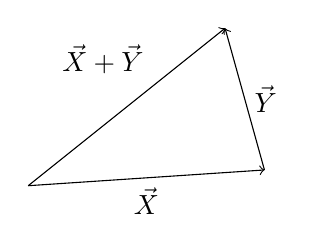
\begin{tikzpicture}
\draw[->] (0,0) -- (3,0.2) node[midway,below]{$\vec{X}$};
\draw[->] (3,0.2) -- (2.5,2) node[midway,right]{$\vec{Y}$};
\draw[->] (0,0) -- (2.5,2) node[midway,above,shift={(-.3,.3)}]{$\vec{X} + \vec{Y}$};
\end{tikzpicture}
\end{marginfigure}
%
\beq
\abs{\vec{X}} + \abs{\vec{Y}} \geq \abs{\vec{X}+\vec{Y}}.
\label{eq:triangle}
\eeq
What is the equivalent of this for our vector space? We need to replace the 3-vectors with kets and work out the magnitudes. Since $\abs{\vec{X}} = \sqrt{x^2+y^2+z^2}$, we need to define a similar magnitude for our kets: $\abs{X}\equiv\sqrt{\avg{X|X}}$. We'll square both sides of Eq.~(\ref{eq:triangle}) to simplify all the square roots.\arnote{Work out the quadratic expansion and simplify.}
\bas
\left(\abs{\vec{X}} + \abs{\vec{Y}}\right)^2 &\geq \abs{\vec{X}+\vec{Y}}^2 \\
\downarrow \phantom{space} & \phantom{space}\downarrow \nonumber\\
\avg{X|X} + \avg{Y|Y} + 2\sqrt{\avg{X|X}\avg{Y|Y}} & \geq \abs{\avg{X|X} +  \avg{Y|Y} + \avg{X|Y} + \avg{Y|X}} \\
\downarrow \phantom{space} & \phantom{space}\downarrow \nonumber\\
 2\sqrt{\avg{X|X}\avg{Y|Y}} & \geq \abs{\avg{X|Y} + \avg{Y|X}} \label{eq:csineq}
\eas
This is one form of the Cauchy-Schwarz inequality. We'll use it to connect the measurement uncertainties of two different observables.

\section{Uncertainty Principle}
\label{sec:generaluncertaintysection}
We now define our state vectors as the output of two different observables $\hat{A}$ and $\hat{B}$ acting on a single input state:
\bas
\ket{X} =& \hat{A}\ket{\Psi} \\
\ket{Y} =&\I \hat{B}\ket{\Psi}.
\eas
We insert these into Eq~(\ref{eq:csineq}) and simplify to get \arnote{Of course you need to work this out. Don't forget that our observables are Hermitian and the definition of the commutator.}
\beq
2\sqrt{\avg{\hat{A}^2}\avg{\hat{B}^2}} \geq \abs{\bra{\Psi}\com{\hat{A},\hat{B}}\ket{\Psi}}.
\label{eq:uncert1}
\eeq

Suppose that both $\avg{\hat{A}}=0$ and $\avg{\hat{B}}=0$. Then the uncertainty of $\Delta A$ is just $\sqrt{\avg{\hat{A}^2}}$ and the same for $\hat{B}$. If this is the case, then we get\toolnote{\toollabel{tool:genuncert}{\includegraphics{tool10.tikz} {\bf Generalized Uncertainty Relationshipper}}  This tool is used to find the uncertainty relationship between two operators.}
\beq
\Delta A \Delta B \geq \frac{1}{2} \abs{\bra{\Psi}\com{\hat{A},\hat{B}}\ket{\Psi}}.
\label{eq:genuncert}
\eeq
This is a general statement of how to consider the combined measurement uncertainties. If we try and measure {\em both} observables, there is a chance that their uncertainties will be related following this relationship. However, if the commutator is zero, then it may be possible to measure both observables with arbitrary precision.

What if $\avg{\hat{A}}\neq0$ and $\avg{\hat{B}}\neq0$? There is a quick trick that can will still make this work. Define two ``shifted'' operators:
\bas
\hat{A}_S =& \hat{A} - \avg{\hat{A}}\\
\hat{B}_S =& \hat{B} - \avg{\hat{B}}.
\eas
We now plug these into the general uncertainty statement and find that Eq.~(\ref{eq:uncert1}) can again be simplified to Eq.~(\ref{eq:genuncert}).\arnote[-0.5cm]{Plug these in and make sure it all works out.}

\begin{example}
What is the relationship between the measurement uncertainties of $\hat{S}_z$ and $\hat{S}_x$ for a single spin initially in the ${+y}$-orientation?

\model We want to know if we can measure both $SG\hat{z}$ and $SG\hat{x}$ like in Exercise~\ref{threeSGs}. So we model these as observables and we'll look for the combined uncertainty.

\vis Our setup is the same as in Exercise~\ref{threeSGs}:
\begin{figure}
\centering
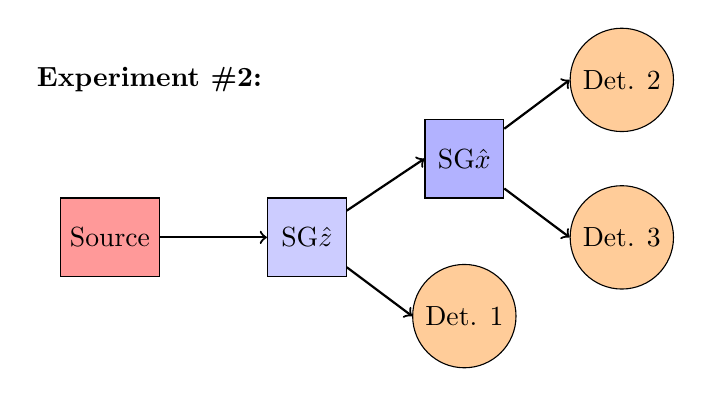
\begin{tikzpicture}
\node at (0,2) {\bf Experiment \#2:};
\node[fill=red!40,shape=rectangle,draw,minimum size=1cm](S) at (-0.5,0){Source};
\node[fill=blue!20,shape=rectangle,draw,minimum size=1cm](SG1) at (2,0){SG$\hat{z}$};
\draw[->,thick] (S) -- (SG1);
\node[fill=blue!30,shape=rectangle,draw,minimum size=1cm](SG2) at (4,1){SG$\hat{x}$};
\draw[->,thick] (SG1) -- (SG2.west);
\node[fill=orange!40,shape=circle,draw](D1) at (4,-1){Det. $1$};
\draw[->,thick] (SG1) -- (D1.west);
\node[fill=orange!40,shape=circle,draw](D2) at (6,2){Det. $2$};
\node[fill=orange!40,shape=circle,draw](D3) at (6,0){Det. $3$};
\draw[->,thick] (SG2) -- (D2.west);
\draw[->,thick] (SG2) -- (D3.west);
\end{tikzpicture}
\end{figure}

\sol We need to know the commutator between the two observables. We saw in Example~\ref{ex:spincommutator} that $\com{\hat{S}_z,\hat{S}_x} = \I\hbar\hat{S}_y$. So in this case if we have an input state $\ket{\Psi}$, the combined uncertainty would be
\beq
\Delta S_z \Delta S_x \geq\frac{1}{2}\abs{\I\hbar\bra{\Psi}\hat{S}_y\ket{\Psi}},
\eeq
which depends on the input state. For example if we input $\ket{\Psi} = \ket{i}$, then the expectation value is
\beq
\bra{i}\hat{S}_y\ket{i} = \frac{\hbar}{2}
\eeq
and the combined uncertainty is
\beq
\Delta S_z \Delta S_x \geq\frac{\hbar^2}{4}.
\eeq
\assess This agrees with the ideas of our Quantum Propositions back in Section~\ref{sec:quantprop}. We found that we couldn't make precise measurements on two different polarization state observables. This is saying the same thing: we are limited in how much we can know when we try and measure both $\hat{S}_z$ and $\hat{S}_x$ on our initial state $\ket{u}$. 

\end{example}

\begin{exercise}
What are the combined measurement uncertainties of  $\hat{S}_z$ and $\hat{S}_x$ for the $x$-direction, $z$-direction and the other $y$-direction input states?
\end{exercise}


\begin{exercise}
Given the Hamiltonian 
\beq
\hat{H} \Meq  E_1 \begin{pmatrix} 1&0&0\\0&2&0\\0&0&2
\end{pmatrix}
\eeq
and the observable
\beq
\hat{B} \Meq  b_1 \begin{pmatrix} 0&1&0\\1&0&0\\0&0&1
\end{pmatrix},
\eeq
\begin{itemize}
\item[(a)] What is the joint uncertainty $\Delta H \Delta B$ for the three input states:
\beq
\ket{1}\Meq  \begin{pmatrix}1\\0\\0\end{pmatrix} \;\ket{2}\Meq  \begin{pmatrix}0\\1\\0\end{pmatrix} \rmt{ and } \ket{3}\Meq  \begin{pmatrix}0\\0\\1\end{pmatrix}?
\eeq
\item[(b)] What is the joint uncertainty for the input state
\beq
\ket{\Psi} \Meq \frac{1}{\stwo}\begin{pmatrix}1\\ \I \\0\end{pmatrix}?
\eeq
\end{itemize}
\end{exercise}

\section{Energy-Time Uncertainty Relationship}

We have another tool we can use to build a better qualitative picture of our quantum system, especially for quantum systems that change with time. We described before how to evaluate the time evolution of the expectation value of an observable in Eq.~(\ref{eq:timeop}) (ignoring any explicit time dependence of the operator):
\beq
\frac{d}{dt}\avg{\hat{L}}  =  \frac{\I}{\hbar}\avg{\com{\hat{H},\hat{L}}}.
\eeq
What happens if $\com{\hat{H},\hat{L}}\neq0$? That means that $\avg{\hat{L}}$ is changing with time. We define a characteristic time scale over which that change happens:
\beq
\Delta t \equiv \frac{\Delta L}{\abs{d\avg{\hat{L}}/dt}}
\eeq
where $\Delta L$ is the measurement uncertainty of the observable. This means that it takes time $\Delta t$ for the observable to change enough for us to be able to measure the change. We combine this with the fact that the Hamiltonian operator measures the energy of a system, $\avg{\hat{H}} = E$ and $\Delta H = \Delta E$. Putting these both into Eq.~(\ref{eq:genuncert}), we get
%
\beq
\Delta E \Delta t \geq \frac{\hbar}{2}.
\label{eq:turel}
\eeq 
\arnote[-0.5cm]{Make sure you follow all the skipped steps here.}
%
So if we know either the time scale or the energy scale of the change, we can find the other. This is something of an approximation, though, because it is often hard to determine the scales of change for any particular system. But as a rule of thumb, Eq.~(\ref{eq:turel}) works to give a general scale.
\begin{example}
What is the approximate time scale for a system that has a measured energy uncertainty of $3.5\times10^{-9}$~eV?

\model We model the energy measurement as a quantum system with $\Delta E=3.5\times10^{-9}$~eV. We are interested in the time scale of whatever observable caused this change.

\vis The uncertainty in energy could look something like this (Figure \ref{fig:samplefig1})
\begin{figure}
\centering
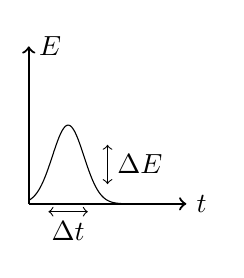
\begin{tikzpicture}
\draw[->,thick] (0,0) -- (2,0) node[right]{$t$};
\draw[->,thick] (0,0) -- (0,2) node[right]{$E$};

\draw[domain=0:2,samples=100] plot({\x},{exp(-(\x-.5)^2/(2*0.2^2))});
\draw[<->] (.25,-.1) -- (.75,-.1) node[midway,below]{$\Delta t$};
\draw[<->] (1,0.25) -- (1,.75) node[midway,right]{$\Delta E$};

\end{tikzpicture}
\caption[][2cm]{ }
\label{fig:samplefig1}
\end{figure}

\sol The time scale is approximately 
\beq
\Delta t \sim \frac{\hbar}{2\Delta E} \sim 94\;\rmt{nanoseconds.}
\eeq

\assess The time scale is reasonable for atomic systems. In terms of a frequency scale, if we look at $\Delta E = h\Delta f$, we find that $\Delta f \approx 850$~kHz, which is typical for atomic systems. That gives us a feel for the energy uncertainties of this type of system.

\end{example}

\begin{exercise}

\begin{enumerate}
\item[(a)]  The half-life of $^{14}$C  is about 5730 years.  Estimate the uncertainty in the energy of  $^{14}$C.  Express your answer in eV.
\item[(b)]   The lifetime of the hydrogen $2p$ excited state, which decays into the $1s$ ground state,  is about $1.6 \times 10^{-9}$~s.   Determine the uncertainty in the energy of the $2p$ state.  Express your answer in eV.
\end{enumerate}
\end{exercise}

\begin{exercise}
 Suppose you are given a beam of spin-1/2 atoms prepared in the state 
%
\beq
\ket{\Psi} = \frac{1}{2}\ket{u} + \I\frac{\sqrt{3}}{2}\ket{d}.
\eeq
%
\begin{enumerate}
\item[(a)] If you measure $\hat{S}_{x}$, find the average and uncertainty of the results.
\item[(b)] If you measure $\hat{S}_{y}$, find the average and uncertainty of the results.
\item[(c)]  Show that your answers to the previous parts are consistent with the generalized uncertainty principle, Eq.~(\ref{eq:genuncert}).

\end{enumerate}
\end{exercise}


\chapter{Multiple Quantum Systems}
\label{ch:mqs}
We've talked about how to describe a single system with multiple observables, creating a CSCO. What if, instead, we want to describe multiple quantum systems? We consider a system of two non-interacting spins. This system is interesting because it will let us probe one of the most interesting elements of the quantum model: entanglement. So we'll start here and build a model to describe this system.

\section{Tensor Products}
\marginnote{We're following Susskind here}We introduce our two quantum systems which we traditionally name ``Alice'' and ``Bob''. We'll start with a classical version of the combined system and then move to the quantum version. Let's say Alice has a coin with possible states heads, $\ket{H}$, and tails, $\ket{T}$. Bob has a six-sided die with states $\ket{1}\ldots\ket{6}$. The combined state is a tensor product of the two individual states which we denote as
\beq
S_{AB} = \underbrace{S_A \otimes S_B.}_{\substack{\rmt{Space of all}\\\rmt{ possible combinations}}}
\eeq
In this particular case, we have 12 possible combinations, so our space $S_{AB}$ has twelve states. We can write each state in a number of different ways. Technically we should write them as $\ket{H}\otimes\ket{3}$ but that gets old after awhile. We could write them as $\ket{H}\ket{3}$, but it is even easier to write the combined state as $\ket{H3}$. The trick to keeping this notation straight is that we have to keep the ordering consistent throughout. We will always write the states as $\ket{\rmt{Alice }\rmt{Bob}}$.

When we take the inner product of two different states in this combined system, we only have states from the same sub-system act on each other. This means that
\beq
\left(\bra{H}\otimes\bra{3}\right)\left(\ket{T}\otimes\ket{4}\right) = \avg{H|T}\otimes\avg{3|4}.
\eeq

Now we can describe the combined system with states like $\alpha_{H3}\ket{H3} + \alpha_{T6}\ket{T6}$. Each one of the twelve possible combinations in $S_{AB}$ is a single state of our system.

\section{Quantum States}
Ok, let's do this now with quantum systems. We will again call our two polarization states ``Alice'' and ``Bob'' and write them as $\ket{ab}$, keeping the ordering straight. The states are orthonormal such that\arnote{Work this out using the expanded tensor product notation.}
\beq
\avg{ab|a'b'} = \delta_{aa'}\delta_{bb'}.
\eeq
We also define the expectation value of an operator $\hat{M}$ acting in this space. The operator could conceivably act on any one of the substates, so we have 
\beq
\bra{ab}\hat{M}\ket{a'b'} = M_{a'b'ab}
\eeq
where the rows of the matrix are labeled as $a'b'$ and the columns as $ab$.

We can expand an arbitrary quantum state in terms of this combined set of basis states:
\beq
\ket{\Psi} = \sum_{ab}\alpha_{ab}\ket{ab}
\label{eq:compound}
\eeq
\marginnote[-1cm]{\ref{tool:decom}}
with combined coefficients $\alpha_{ab}$ of both $a$ and $b$ together.

What if Alice and Bob each have their own measurement system? In that case, the operators might not be combined, but might only act on one or the other states. For example, if we are talking about polarization states, Alice could measure her state which we model as the operators $\hat{\sigma}_1$, $\hat{\sigma}_2$, and $\hat{\sigma}_3$. Bob could do the same thing, but we'll model his measurements as the operators $\hat{\tau}_1$, $\hat{\tau}_2$, and $\hat{\tau}_3$ to keep them different from Alice's measurements. We will work in the $V-H$-basis for both Alice and Bob, just to keep things easy. In this basis, there are four possible states:\marginnote{Remember we've written these as $\ket{\rmt{Alice Bob}}$.}
\beq
\ket{VV},\;\ket{VH},\;\ket{HV},\;\rmt{and }\ket{HH}.
\eeq
When only one person's operator acts on one of these combined states, we leave the other state alone --- it just goes along for the ride. So our notation is like this:\marginnote{We should technically write this as $\hat{\sigma}_3\otimes\onehat$. Then we use the pattern $(\hat{A}\otimes\hat{B})(\ket{a}\otimes\ket{b}) = \hat{A}\ket{a}\otimes\hat{B}\ket{b}$.}
\bas
\hat{\sigma}_3\ket{VV} &= \left(\hat{\sigma}_3\ket{V}\right)\otimes\ket{V} = +1\ket{VV}\\
\hat{\tau}_3\ket{VV} &= \ket{V}\otimes\left(\hat{\tau}_3\ket{V}\right) = +1\ket{VV}.
\eas

\section{Product States}
One type of combined system could be a {\em product state} which is composed of two states, joined together. For example, Alice could have a state $\alpha_V\ket{V} + \alpha_H\ket{H}$ and Bob could have a state $\beta_V\ket{V} + \beta_H\ket{H}$. The product state is just the tensor product of these two states:
\bas
\ket{\Psi}_\rmt{prod} =& \left(\alpha_V\ket{V} + \alpha_H\ket{H} \right) \otimes \left(\beta_V\ket{V} + \beta_H\ket{H} \right)\\
{} = & \alpha_V\beta_V\ket{VV} + \alpha_H\beta_V\ket{HV}  +  \alpha_V\beta_H\ket{VH} + \alpha_H\beta_H\ket{HH}.
\eas
As you can see, there are four possible states and we need four coefficients to describe the product state. It may look like there are more because all four are complex numbers, but there are two normalization conditions plus two unimportant phases, so the number of parameters really is four.

\begin{example}
Alice and Bob have prepared the initial polarization state
\beq
\ket{\Psi} = \frac{\I}{2\sqrt{3}}\ket{VV} + \frac{1}{2}\ket{VH} - \sqrt{\frac{1}{6}}\ket{HV} + \frac{\I}{\sqrt{2}}\ket{HH}
\eeq
Is this a product state? Is it normalized? If Alice and Bob each measure their ElMaWs using a PBS and no waveplates, what would each of them measure on average for many identically prepared states?

\model We model both Alice's and Bob's ElMaWs as quantum states. We need to know what each of them have individually to find their average measurements. We'll model the polarization measurement as the $\hat{\sigma}_3$ and $\hat{\tau}_3$ operators for Alice and Bob, respectively.

\vis This is a combined system with two separate measurements. We model the polarization measurements in an abstract way like we've done with spin measurements.
\begin{figure}
\centering
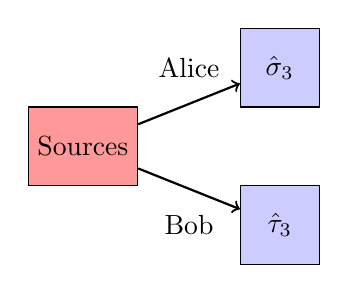
\begin{tikzpicture}
\node[fill=red!40,shape=rectangle,draw,minimum size=1cm](S) at (-0.5,0){Sources};
\node[fill=blue!20,shape=rectangle,draw,minimum size=1cm](SG1) at (2,1){$\hat{\sigma}_3$};
\draw[->,thick] (S) -- (SG1)node[midway,above,shift={(0,.2)}]{Alice};
\node[fill=blue!20,shape=rectangle,draw,minimum size=1cm](SG2) at (2,-1){$\hat{\tau}_3$};
\draw[->,thick] (S) -- (SG2)node[midway,below,shift={(0,-.2)}]{Bob};
\end{tikzpicture}
\end{figure}

\sol We need to know if the state can be written as the product of two individual spin states. It factors as
\beq
\frac{1}{6}\left(\I\sqrt{3}\ket{V} + 3\ket{H}\right)\otimes\left(\ket{V} + \I\sqrt{2}\ket{H}\right).
\eeq
We need both states to be normalized, so that $1/6$ in front needs to be split into \arnote{You try this. Maybe use your \CAS and a \texttt{Factor} function.}
\beq
\left(\frac{\I}{2}\ket{V} + \frac{\sqrt{3}}{2}\ket{H}\right)\otimes\left(\frac{1}{\sqrt{3}}\ket{V} + \I\sqrt{\frac{2}{3}}\ket{H}\right).
\eeq
That is a product state that is normalized. Alice measures an average of $-1/2$ and Bob measures and average of $-1/3$.
\marginnote{\ref{tool:avg}}

\assess Both Alice and Bob have a mostly $\ket{H}$ state, so we expect the averages to be negative. That makes sense.

\end{example}

\begin{exercise}
Alice and Bob have prepared the initial atomic spin state
\beq
\ket{\Psi} = \frac{4\I}{3\sqrt{5}}\ket{uu} - \frac{2}{3}\ket{ud} + \frac{2}{3\sqrt{5}}\ket{du} + \frac{\I}{3}\ket{dd}
\eeq
Is this a product state? Is it normalized? If Alice and Bob each measure their spins using a magnetic field gradient pointed in the $z$-direction, what would each of them measure on average for many identically prepared atoms?
\end{exercise}

\section{Entangled States}

Since we have the freedom to choose four parameters to describe the general quantum state of two combined ElMaWs, what if we choose the parameters to give us the following combined state:\marginnote{This state can be produced using a technique called {\em parametric downconversion}. A laser is directed into a nonlinear crystal that responds by producing the entangled state of two quantum ElMaWs.}
\beq
\ket{\Psi_s} = \frac{1}{\stwo}\left(\ket{VH} - \ket{HV}\right)?
\eeq
The first thing we notice is that this state can't be factored into two separate product states. That makes it an {\em entangled} state. There are an infinite number of possibilities for entangled states, but a few of them are particularly interesting and this is one of those. We call this state a {\em singlet} entangled state. Let's look at the properties of this state. First, what do Alice's and Bob's measure if they average a number of polarization measurements?
\begin{example}
What are the average measurements of $\hat{\sigma}_1$, $\hat{\sigma}_2$, and $\hat{\sigma}_3$ for the singlet state?
\beq
\ket{\Psi_s} = \frac{1}{\stwo}\left(\ket{VH} - \ket{HV}\right)
\eeq

\model Even though this entangle state can't be {\em written} as two product states, that doen't mean that the ElMaWs are connected. Alice and Bob still each have their own waves and can make their measurements. So we model their ElMaWs as separate with separate measurements. We model the polarization measurement as a linear operator in the $V-H$ basis and look at Alice's averages.

\vis Alice measures her half of the combined state. We assume Bob can measure his, too.
\begin{figure}
\centering
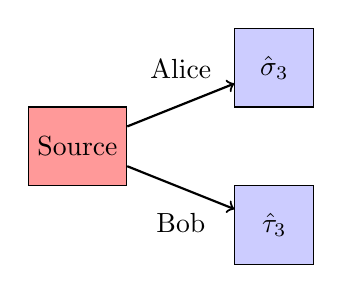
\begin{tikzpicture}
\node[fill=red!40,shape=rectangle,draw,minimum size=1cm](S) at (-0.5,0){Source};
\node[fill=blue!20,shape=rectangle,draw,minimum size=1cm](SG1) at (2,1){$\hat{\sigma}_3$};
\draw[->,thick] (S) -- (SG1)node[midway,above,shift={(0,.2)}]{Alice};
\node[fill=blue!20,shape=rectangle,draw,minimum size=1cm](SG2) at (2,-1){$\hat{\tau}_3$};
\draw[->,thick] (S) -- (SG2)node[midway,below,shift={(0,-.2)}]{Bob};
\end{tikzpicture}
\end{figure}

\sol We need to know how the polarization measurement operators act on the different input polarization states. Looking at Alice's states alone we've got \arnote{Use the matrix representation to check these.}
\bas
\hat{\sigma}_1\ket{V} & = \ket{H} & \hat{\sigma}_1\ket{H} & = \ket{V} \\ 
\hat{\sigma}_2\ket{V} & = \I\ket{H} & \hat{\sigma}_2\ket{H} & = {-\I\ket{V}} \\
\hat{\sigma}_3\ket{V} & = \ket{V} & \hat{\sigma}_3\ket{H} & = {-\ket{H}}.
\eas
So if we let Bob's state go along for the ride, we get
\bas
\hat{\sigma}_1\ket{VH} & = \ket{HH} & \hat{\sigma}_1\ket{HV} & = \ket{VV} \\ 
\hat{\sigma}_2\ket{VH} & = \I\ket{HH} & \hat{\sigma}_2\ket{HV} & = {-\I\ket{VV}} \\
\hat{\sigma}_3\ket{VH} & = \ket{VH} & \hat{\sigma}_3\ket{HV} & = {-\ket{HV}}.
\eas
So we get\arnote{Check these, too, to make sure you can do them all yourself.}
\bas
\bra{\Psi_s}\hat{\sigma}_1\ket{\Psi_s} = & 0 \\ 
\bra{\Psi_s}\hat{\sigma}_2\ket{\Psi_s} = & 0 \\ 
\bra{\Psi_s}\hat{\sigma}_3\ket{\Psi_s} = & 0 
\eas

\assess This would be the same result if we measured Bob's polarizations, too. This is interesting because it means that the ``polarization'' of the singlet state doesn't ``point'' along any direction at all. We would expect that one or more of these would be zero. In fact we expect that
\beq
\avg{\hat{\sigma}_1}^2 + \avg{\hat{\sigma}_2}^2 + \avg{\hat{\sigma}_3}^2 = 1
\eeq
which obviously isn't the case for our entangled state.
\end{example}

\begin{exercise}
What are the average measurements of $\hat{S}_x$, $\hat{S}_y$, and $\hat{S}_z$ for the input spin state (in the $z$ basis)
\beq
\ket{\Psi_{T0}} = \frac{1}{\stwo}\left(\ket{ud} + \ket{du}\right)?
\eeq
\end{exercise}

\section{Correlations}
\label{sec:covariance}
Early on we looked at the idea of correlations (See Section~\ref{sec:correlation}). We return to that idea and look at the correlations between Alice's and Bob's states. Before doing this with the quantum states, let's look at a classical version.

\subsection{Classical Correlations}
We are going to enlist a third person, Charlie, who has two coins: one of them red and one blue. Each red coin has a ``$+1$'' labeled on it and each blue coin has a ``$-1$''.\begin{marginfigure}
\begin{tikzpicture}
  \node[name=A,cylinder,draw=black,thick,minimum width=1.5cm,aspect=3,shape border rotate=90,cylinder uses custom fill, cylinder body fill=red!30,cylinder end fill=red!40,label={[shift={(0,-0.6)}]north:$+1$}] at (0,0) {};
    \node[name=B,cylinder,draw=black,thick,minimum width=1.5cm,aspect=3,shape border rotate=90,cylinder uses custom fill, cylinder body fill=blue!30,cylinder end fill=blue!40,label={[shift={(0,-0.6)}]north:$-1$}] at (3,0) {};
\end{tikzpicture}
\end{marginfigure}
Charlie mixes up the coins and then hands one to Alice and one to Bob. Nobody looks at the coins at this point. Alice then gets on a ship and travels across the galaxy. When she gets to the other side she looks at her coin. She immediately knows which color coin Bob has, even though he is on the other side of the galaxy. Of course relativity hasn't been violated here --- Alice's knowledge has not transmitted any information. If she were to try and tell Bob what color coin he has before he looks at it, she would have to send a classical signal at the speed of light.

We now repeat this experiment many times with many Alice and Bob pairs. Over time each of them average out their measurements. Alice's average measurement (which we'll call $\sigma_A$) (assuming that Charlie is randomly handing out coins) is $\avg{\sigma_A}=0$ as is Bob's ($\avg{\sigma_B}=0$). However, what if we measure the product of their measurements? Every time Alice measures a red coin, she knows Bob measures a blue, and vice-versa. So the average of the product is always
\beq
\avg{\sigma_A\sigma_B}=-1.
\eeq
The definition of a statistical covariance is\marginnote{Note the similarity to the second-order correlation from Section \ref{sec:correlation}. This is a related measure.} 
\beq
\rmt{cov}(A,B)=\avg{\sigma_A\sigma_B} - \avg{\sigma_A}\avg{\sigma_B}.
\eeq
If this is zero the measurements are uncorrelated. Our situation has a covariance of $-1$, so the two states are correlated. The correlation comes from the fact that Charlie set up the correlation to begin with, so it isn't too surprising.

\subsection{Quantum Correlation}
We can do the same thing with our combined quantum system. Alice and Bob each need to measure their states independently. We also need to have them get together afterwards and compare their measurements to calculate the covariance. To do this, we need a combined operator 
$\hat{\sigma}_3\hat{\tau}_3$. The way this combined operator works is that Alice's operator $\hat{\sigma}_3$ only acts on her state and Bob's operator $\hat{\tau}_3$ only acts on his. The formal notation for this (which we've seen before) is
\beq \left(\hat{A}\otimes\hat{B}\right)\left(\ket{a}\otimes\ket{b}\right) = \hat{A}\ket{a}\otimes \hat{B}\ket{b}.
\label{eq:compop}
\eeq
\marginnote[-1cm]{For example $\hat{\sigma}_3\hat{\tau}_3\ket{VV} = \ket{VV}$ and $\hat{\sigma}_3\hat{\tau}_3\ket{VH} = -\ket{VH}$. } 
We'll come back to this idea in a little bit and use it to look at another test for entanglement.


\begin{example}
What is the covariance of Alice's and Bob's measurements of the following two polarization states if both Alice and Bob measure for $V-H$ polarization?  
\bas
\ket{\Psi_s} &= \frac{1}{\stwo}\left(\ket{VH}-\ket{HV}\right) \\
\ket{\Psi_2} &= \frac{1}{\stwo}\left(\ket{VH}-\ket{VV}\right)
\eas

\model We model Alice's measurement as the operator $\hat{\sigma}_3$ and Bob's as $\hat{\tau}_3$. 

\vis Alice measures her half of the combined state and Bob measure's his.
\begin{figure}
\centering
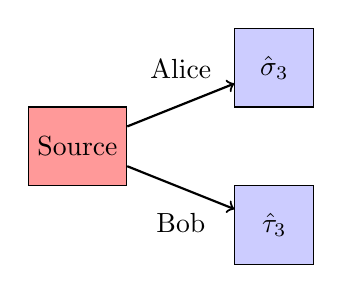
\begin{tikzpicture}
\node[fill=red!40,shape=rectangle,draw,minimum size=1cm](S) at (-0.5,0){Source};
\node[fill=blue!20,shape=rectangle,draw,minimum size=1cm](SG1) at (2,1){$\hat{\sigma}_3$};
\draw[->,thick] (S) -- (SG1)node[midway,above,shift={(0,.2)}]{Alice};
\node[fill=blue!20,shape=rectangle,draw,minimum size=1cm](SG2) at (2,-1){$\hat{\tau}_3$};
\draw[->,thick] (S) -- (SG2)node[midway,below,shift={(0,-.2)}]{Bob};
\end{tikzpicture}
\end{figure}

\sol We already know that $\bra{\Psi_s}\hat{\sigma}_3\ket{\Psi_s}=0$ and $\bra{\Psi_s}\hat{\tau}_3\ket{\Psi_s}=0$. We need to find the averages for the other state, though. They are\arnote{Lots to work through here. Make sure you get the same answers!}%
\bas
\bra{\Psi_2}\hat{\sigma}_3\ket{\Psi_2}=&1\\
\bra{\Psi_2}\hat{\tau}_3\ket{\Psi_2}=&0.
\eas
We also need the combined operator average. It is 
\bas
\bra{\Psi_s}\hat{\sigma}_3\hat{\tau}_3\ket{\Psi_s}=&-1\\
\bra{\Psi_2}\hat{\sigma}_3\hat{\tau}_3\ket{\Psi_2}=&0.
\eas
So we have
\bas
\rmt{cov for } \ket{\Psi_s} \rightarrow &  -1 + 0\cdot0 = -1\\
\rmt{cov for } \ket{\Psi_2} \rightarrow &  0 + 0\cdot1 = 0.
\eas

\assess The singlet state $\ket{\Psi_s}$ is an entangled state and has a non-zero covariance. That means that Alice's and Bob's measurements are correlated. The other state, $\ket{\Psi_2}$, however, is a product state. Its covariance is zero and is uncorrelated. \marginnote{This is the first test for entanglement. If the covariance is nonzero than the state has some degree of entanglement.}

\end{example}

\begin{exercise}
What is the covariance (measured in the $z$-direction) if Charlie prepares two atomic spins in the following states and gives them to Alice and Bob to measure:
\beq
\ket{\Psi_{T0}} = \frac{1}{\stwo}\left(\ket{ud}+\ket{du}\right) ?
\eeq
\end{exercise}

\begin{exercise}
What are the covariances in the other two directions ($x$ and $y$) for the same state?
\beq
\ket{\Psi_{T0}} = \frac{1}{\stwo}\left(\ket{ud}+\ket{du}\right)
\eeq
\end{exercise}




\chapter{Composite Operators}
Our use of composite operators was a little bit clunky - it would be nice to have a new set of tools that lets us generalize the types of measurements and interactions we can do on our composite states. We are going to work in a matrix representation in order to make these new tools.

In creating our combined states we defined the matrix elements of our operators as 
\beq
\bra{ab}\hat{M}\ket{a'b'} = M_{a'b'ab}
\eeq
where the rows of the matrix are label as $a'b'$ and the columns as $ab$. Working with the polarization states and their matrix representation, we'll try building a matrix representation for Alice's $\hat{\sigma}_3$ operator where Bob does nothing (which is the $\onehat$ operator) using the $V-H$ basis. We'll combine our two states and represent them as\marginnote{So in this basis 
\bas
\ket{VV} &\Meq  \begin{pmatrix}1\\0\\0\\0\end{pmatrix},& 
\ket{VH} &\Meq  \begin{pmatrix}0\\1\\0\\0\end{pmatrix}, \\
\ket{HV} &\Meq  \begin{pmatrix}0\\0\\1\\0\end{pmatrix}, &  
\ket{HH} &\Meq  \begin{pmatrix}0\\0\\0\\1\end{pmatrix}.
\eas}
\beq
\ket{AB}=\ket{A}\otimes\ket{B} \Meq  \vket{a_{11}
}{a_{12}} \otimes \vket{b_{11}
}{b_{12}} = \begin{pmatrix}a_{11}b_{11}\\a_{11}b_{12}\\a_{21}b_{11}\\a_{21}b_{21}\end{pmatrix}.
\eeq
%
In tensor product notation, we want
$\hat{A}\otimes\hat{B}$.
\beq
\hat{A}\otimes\hat{B} \Meq  \begin{pmatrix}\highlight[h1color]{A_{11}\hat{B}}&\highlight[h2color]{A_{12}\hat{B}}\\
\highlight[h3color]{A_{21}\hat{B}}&\highlight[h4color]{A_{22}\hat{B}}\end{pmatrix} = 
\begin{pmatrix}\highlight[h1color]{
\begin{matrix}A_{11}B_{11}&A_{11}B_{12}\\
A_{11}B_{21}&A_{11}B_{22} \end{matrix}} &
\highlight[h2color]{\begin{matrix}A_{12}B_{11}&A_{12}B_{12}\\
A_{12}B_{21}&A_{12}B_{22} \end{matrix}}\\
\highlight[h3color]{
\begin{matrix}A_{21}B_{11}&A_{21}B_{12}\\
A_{21}B_{21}&A_{21}B_{22} \end{matrix}} &
\highlight[h4color]{\begin{matrix}A_{22}B_{11}&A_{22}B_{12}\\
A_{22}B_{21}&A_{22}B_{22} \end{matrix}}
\end{pmatrix}
\eeq
So our specific case means that $\hat{\sigma}_3\otimes\onehat$ becomes\arnote{Check that this combined operator acts on the four combined states the way it should.}
\beq
\hat{\sigma}_3\otimes\onehat \Meq  \begin{pmatrix}
1&0&0&0\\
0&1&0&0\\
0&0&-1&0\\
0&0&0&-1
\end{pmatrix}.
\eeq
This gives us the same result in the matrix representation as we defined in Eq.~(\ref{eq:compop}).
\begin{exercise}
Alice and Bob have two atomic spins and want to make all the possible separate measurements on their systems. What is the matrix representations for $\hat{S}_x\otimes\hat{T}_y$ (where $\hat{T}_y$ is Bob's model for his spin measurement)? How about the other combined directions?
\end{exercise}


\section{Math Interlude: Outer Products}
We need a new mathematical tool now. We define the {\em outer product} of two quantum states as
\beq
\oprod{\Psi}{\Phi}.
\eeq
Note that the ordering as I've written it here is important. It is like a bra-ket but backwards: it is a ket-bra. As such it is an operator. It acts on quantum states and the output is another quantum state. We use it like this:
\bas
\oprod{\Psi}{\Phi}\;\ket{A} & = \ket{\Psi}\avg{\Phi|A}\\
\bra{B}\;\oprod{\Psi}{\Phi} & = \avg{B|\Psi}\bra{\Phi}.
\eas

A specific version of the outer product is known as the projection operator which is just the same state in an outer product: $\ket{\Psi}\bra{\Psi}$. This has the property that it evaluates how much a different state ``lies along'' the states $\ket{\Psi}$.\marginnote{This is similar to the dot product for 3-vectors.} So if we evaluate 
\beq
\oprod{\Psi}{\Psi}\; \ket{A} = \ket{\Psi}\avg{\Psi|A}
\eeq
we get a new ket-vector that is similar to the projection operator. The projection operator has a couple of useful properties:
\begin{itemize}
\item It is Hermitian: $\left(\oprod{\Psi}{\Psi}\right)^\dagger = \oprod{\Psi}{\Psi}$.
\item $\ket{\Psi}$ is an eigenvector with eigenvalue of $1$: $\left(\oprod{\Psi}{\Psi}\right)\;\ket{\Psi} = \ket{\Psi}$.
\item If $\avg{\Psi|\Phi}=0$ then $\ket{\Phi}$ is an eigenvector with eigenvalue of $0$.
\item The projection operator squared is itself: $\left(\oprod{\Psi}{\Psi}\right)^2=\oprod{\Psi}{\Psi}$
\end{itemize}

\begin{example}
A single atom spin is prepared in the state
\beq
\ket{\Psi} = \frac{1}{2}\ket{u} + \frac{\I\sqrt{3}}{2}
\ket{d}.
\eeq
Show that the properties of the projection operator work for this state.

\model We're working in the $z$-basis for a single atom spin. We need to work through all the properties.

\vis Here's looking at you, kid.

\sol The projection operator, written out, is
\beq
\oprod{\Psi}{\Psi} = \frac{1}{4}\oprod{u}{u} - \frac{\I\sqrt{3}}{4}\left(\oprod{u}{d} - \oprod{d}{u}\right) + \frac{3}{4}\oprod{d}{d}.
\eeq
When we take the Hermitian conjugate, we flip the order of the vectors and take the complex conjugate. That gives us\arnote{Work through all of these, filling in the steps.}
\beq
\oprod{\Psi}{\Psi}^\dagger = \frac{1}{4}\oprod{u}{u} + \frac{\I\sqrt{3}}{4}\left(\oprod{d}{u} - \oprod{u}{d}\right) + \frac{3}{4}\oprod{d}{d},
\eeq
which is the same thing. We test that $\ket{\Psi}$ is an eigenvector:
\bas
\oprod{\Psi}{\Psi}\ket{\Psi} = & \left[\frac{1}{4}\oprod{u}{u} + \frac{\I\sqrt{3}}{4}\left(\oprod{d}{u} - \oprod{u}{d}\right) + \frac{3}{4}\oprod{d}{d}\right]\nonumber\\
{} & \left(\frac{1}{2}\ket{u} + \frac{\I\sqrt{3}}{2}\ket{d}\right)\\
= & \frac{1}{8}\ket{u}  + \frac{\I\sqrt{3}}{8}\ket{d} + \frac{3}{8}\ket{u} + \frac{3\I\sqrt{3}}{8}\ket{d}\\
= &\ket{\Psi}
\eas
That works. We'd need an orthogonal vector to test the next one. The easiest to test is $\ket{\Phi} = \I\sqrt{3}/2\ket{u} + 1/2\ket{d}$. With this vector, we find that $\oprod{\Psi}{\Psi}\ket{\Phi}=0$ as expected. Finally, we check that $(\oprod{\Psi}{\Psi})^2 = \oprod{\Psi}{\Psi}$:
\bas
\left(\oprod{\Psi}{\Psi}\right)^2 = & \left[\frac{1}{4}\oprod{u}{u} + \frac{\I\sqrt{3}}{4}\left(\oprod{d}{u} - \oprod{u}{d}\right) + \frac{3}{4}\oprod{d}{d}\right]^2\\
= & \frac{1}{16}\oprod{u}{u} + \frac{\I\sqrt{3}}{16}\oprod{d}{u} + \frac{3}{16}\oprod{u}{u}  + \frac{\I 3\sqrt{3}}{16}\oprod{d}{u} \nonumber\\
{} & - \frac{\I\sqrt{3}}{16}\oprod{u}{d} + \frac{3}{16}\oprod{d}{d} - \frac{\I3\sqrt{3}}{16}\oprod{u}{d}+ \frac{9}{16}\oprod{d}{d}\\
{}= & \oprod{\Psi}{\Psi}.
\eas

\assess Everything worked out as it should.

\end{example}

\begin{exercise}
We prepare a polarization state as
\beq
\ket{\Psi} = \I\sqrt{\frac{3}{5}}\ket{D_R} + \sqrt{\frac{2}{5}}\ket{D_L}.
\eeq
Show that the properties of the projection operator work for this state.
\end{exercise}


\section{The Trace}

The {\em trace} is one more new tool that we need, especially moving forward with building a description of entangled states. We define the trace $\Tr$ as the sum of the diagonal entries in a square matrix.
\beq
\Tr\begin{pmatrix}\highlight[h1color]{1}&5&0&0\\5&\highlight[h1color]{2}&7&-\I\\0&7&\highlight[h1color]{3}&-4\\0&\I&-4&\highlight[h1color]{4}\end{pmatrix} = 1+2+3+4 = 10.
\eeq
Since we can write an operator in terms of its matrix elements in the $\ket{j}$ basis, we define the trace of an operator as
\beq
\Tr\hat{L} = \sum_j\bra{j}\hat{L}\ket{j},
\label{eq:tracedef}
\eeq
where we sum up all the diagonal elements. We saw previously that the diagonal elements of a Hermitian operator were its eigenvalues, so the trace of a Hermitian operator is just the sum of its eigenvalues. And, since the projection operator is Hermitian (with one non-zero eigenvalue), that means that
\beq
\Tr\oprod{\Psi}{\Psi} = 1.
\eeq
And if we add up all of the projection operators in the $\ket{j}$ basis we get\marginnote{We've seen this before as the \ref{tool:span}.}
\beq
\sum_j\oprod{j}{j} = \onehat.
\eeq
Finally, we now write the average measurement of an operator in terms of the trace and the projection operator: \marginnote[1cm]{\ref{tool:span}}
\bas
\bra{\Psi}\hat{L}\ket{\Psi} = & \sum_j \bra{\Psi}\hat{L}\left(\oprod{j}{j} \right) \ket{\Psi} \\
= &\sum_j \avg{j|\Psi}\bra{\Psi}\hat{L}\ket{j}\\
= & \sum_j \bra{j}\left[\oprod{\Psi}{\Psi}\hat{L}\right] \ket{j}\\
= & \Tr \oprod{\Psi}{\Psi}\hat{L}\label{eq:travg}.
\eas\marginnote[-1cm]{This is a new version of \ref{tool:avg}.}
So if we have both the operator of interest and the projection operator in a matrix representation, finding the average measurement of the operator is a matter of doing the matrix multiplication, then taking the trace.

\begin{example}
What is the projection operator for the spin state $\ket{u}$ in the matrix notation? What is $\avg{\hat{S}_y}$?

\model We're modeling a single atomic spin here and we'll be using the $z$-basis to write it using matrix notation.

\vis Did you see that?!?!

\sol The state is 
\beq
\ket{u} \Meq  \vket{1}{0}
\eeq
in matrix notation. So the outer product becomes\marginnote[1cm]{Multiplying two row vectors this direction gives us 
\beq\vket{a_1^{}}{a_2^{}}\vbra{b_1^{*}}{b_2^{*}} = \begin{pmatrix}a_1^{}b_1^{*} & a_1^{}b_2^{*} \\ a_2^{}b_1^{*} & a_2^{}b_2^{*}\end{pmatrix}\eeq}
\beq
\oprod{u}{u}\Meq  \vket{1}{0}\vbra{1}{0} = \begin{pmatrix}1&0\\0&0\end{pmatrix}
\eeq
Now to find the average. In the $z$-basis we have
\beq
\hat{S}_y\Meq  \frac{\hbar}{2}\symatrix.
\eeq
So we need\arnote{Review matrix multiplication and write it out explicitly.}
\bas
\Tr\oprod{u}{u}\hat{S}_y \Meq  & \Tr \begin{pmatrix}1&0\\0&0\end{pmatrix} \frac{\hbar}{2}\symatrix\\
&=\frac{\hbar}{2}\Tr\begin{pmatrix}0&-\I\\0&0\end{pmatrix} \\
&=\frac{\hbar}{2}(0+0) = 0.
\eas


\assess This looks good - the projection matrix is a Hermitian matrix that will satisfy all of the requirements. The average is what we expect.

\end{example}

\begin{exercise}
What is the projection operator for the polarization state $\ket{C_R}$ in matrix notation in the $V-H$ basis?
\end{exercise}

\begin{exercise}
Using the formula in Eq.~(\ref{eq:travg}), what is $\bra{C_R}\hat{\sigma}_2\ket{C_R}$?
\end{exercise}



\chapter{The Density Matrix}
Up to this point we've concentrated on quantum states where we have full knowledge of the input quantum state and everything that happens to the state until we measure it. However, that model doesn't provide us with tools for dealing with real-world situations where we might not have complete control over everything.\marginnote[-1cm]{This is a similar situation to classical mechanics, kinematics, and friction: we start by modeling everything as frictionless, then add in a friction model to make it a better model.} We now build a model that will let us describe that kind of situation.

Going back to Alice, Bob, and Charlie: say Charlie gives us a state, but he doesn't tell us what he's done? Or what if he gives us a state like this:
\beq
\ket{\Psi} = \alpha\ket{A} + \beta\E{\I\theta}\ket{B}
\eeq
but the phase $\theta$ gets scrambled? The loss of phase information is called {\em decoherence} and we'll come back to it in just a bit. \marginnote[-0.5cm]{This happens all the time in the lab with atomic spin states when there are uncontrolled fluctuations in the magnetic field.} What can we still say about the system? Using this new model, there are still predictions we can make even if we have lost information about the entire quantum state.

\section{Density Matrix}
Suppose Charlie gives Alice an atomic spin {\em mixed state} that may be in state $\ket{\Phi}$ with a 50\% probability or it may be in state $\ket{\Psi}$ with 50\% probability. We can't write the state as a {\em pure state}: $\ket{\Psi}=1/\stwo(\ket{\Psi} + \ket{\Phi})$ because that model means that we know the phase relationship between the two states. In this model, we don't know what that phase is, so we can't write it as a pure state. However, Alice knows that if the state Charlie gave her was actually $\ket{\Psi}$, then the average measurement of her operator $\hat{L}$ would be:
\beq
\avg{\hat{L}_\Psi} = \Tr \oprod{\Psi}{\Psi}\hat{L}
\eeq
and if she were given the state $\ket{\Phi}$, the average would be
\beq
\avg{\hat{L}_\Phi} = \Tr \oprod{\Phi}{\Phi}\hat{L}.
\eeq
Since each of these possible averages each have a 50\% chance of happening, the overall average of the state that Charlie gave her is just
\beq
\avg{\hat{L}} = \frac{1}{2}\left(\Tr \oprod{\Psi}{\Psi}\hat{L} \right) + \frac{1}{2}\left(\Tr \oprod{\Phi}{\Phi}\hat{L} \right),
\eeq
\marginnote{Since the probabilities add up to $1$, we know that \beq\sum_nw_n=1.\eeq}where the weight factors $w_n = 1/2$ tell us what the probabilities are of getting each separate result. We now define the {\em density operator} to simplify writing this notation. If we have a collection of possible states $\ket{\Psi_n}$ that our state could be in, each with weight $w_n$, then the density operator is
\beq
\hat{\rho} \equiv \sum_n w_n \oprod{\Psi_n}{\Psi_n}.
\label{eq:densitymat}
\eeq
\marginnote[-0.4cm]{Conventionally the density operator is written as $\hat{\rho}$. Don't confuse it with the polar coordinate 3-vector radial unit vector.} Now the average measurement of Charlie's mixed state is
\beq
\avg{\hat{L}} = \Tr(\hat{\rho}\hat{L}).
\label{eq:densitmatrixavg}
\eeq
This notation has packaged everything that Alice knows about Charlie's state in one neat form. All of our quantum mechanics models and tools can be reformulated in terms of the density matrix\marginnote{The density operator is often called the {\em density matrix}. We mean the same thing.}. We won't do that here because we won't be using those tools, but the Schr\"{o}dinger equation, time evolution, and everything else can all be re-written using the density matrix.


%Is it worth talking about the state of the density operator after measurement? We haven't said anything to this point...

\begin{example}
Charlie gives us an atomic spin state that is either $\ket{d}$ with 30\% probability or is $\ket{o}$ with 70\% probability. What is our density matrix and the average measurement of the spin in the $z$-direction?

\model We'll use the matrix representation for our states, working in the $z$ basis. In this basis we represent the two possible states as 
\beq
\ket{d}\Meq \vket{0}{1}\qquad\ket{o}\Meq \vket{\frac{1}{\stwo}}{\frac{-\I}{\stwo}}.
\eeq
We also need to model our measurement as an operator in this basis. It is
\beq
\hat{S}_z\Meq \frac{\hbar}{2}\szmatrix.
\eeq

\vis Our setup is simple: we're given a state and measure it.
\begin{figure}
\centering
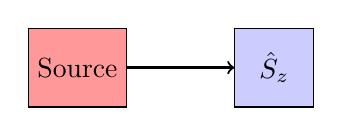
\begin{tikzpicture}
\node[fill=red!40,shape=rectangle,draw,minimum size=1cm](S) at (-0.5,0){Source};
\node[fill=blue!20,shape=rectangle,draw,minimum size=1cm](SG1) at (2,0){$\hat{S}_z$};
\draw[->,thick] (S) -- (SG1);
\end{tikzpicture}
\end{figure}

\sol We need the density operator in our matrix notation. We know the weights, but we need the outer products:
\bas
\oprod{d}{d} \Meq  & \vket{0}{1}\vbra{0}{1} = \begin{pmatrix}0&0\\0&1\end{pmatrix}\\
\qquad\oprod{o}{o}\Meq  & \vket{\frac{1}{\stwo}}{\frac{-\I}{\stwo}}\vbra{\frac{1}{\stwo}}{\frac{\I}{\stwo}} = \begin{pmatrix}\frac{1}{2}&\frac{\I}{2}\\\frac{-\I}{2}&\frac{1}{2}\end{pmatrix}
\eas
So our density operator is
\beq
\hat{\rho}=\sum_n w_n\oprod{\Psi_n}{\Psi_n}\Meq   0.3\begin{pmatrix}0&0\\0&1\end{pmatrix} + 0.7 \begin{pmatrix}\frac{1}{2}&\frac{\I}{2}\\\frac{-\I}{2}&\frac{1}{2}\end{pmatrix}.
\eeq
The average measurement of the spin in the $z$-direction is \arnote{Work through all the matrix multiplications and additions. Make sure you understand how to use the trace.}
\bas
\avg{\hat{S}_z}=\Tr(\hat{\rho}\hat{L})\Meq & \Tr\left[0.3\begin{pmatrix}0&0\\0&1\end{pmatrix} + 0.7 \begin{pmatrix}\frac{1}{2}&\frac{\I}{2}\\\frac{-\I}{2}&\frac{1}{2}\end{pmatrix} \right]\frac{\hbar}{2}\szmatrix \\
&=\frac{\hbar}{2}\Tr\left[0.3\begin{pmatrix}0&0\\0&-1\end{pmatrix} + 0.7 \begin{pmatrix}\frac{1}{2}&\frac{-\I}{2}\\\frac{-\I}{2}&\frac{-1}{2}\end{pmatrix}   \right] \\
&=\frac{\hbar}{2}\Tr\begin{pmatrix}0.35&-0.35\I\\-0.35\I&-.65\end{pmatrix}\\
&=\frac{\hbar}{2}(.35-.65) = -.15\hbar.
\eas

\assess If Charlie had given us 100\% $\ket{o}$, the average would have been $0$. So the fact that he gave us a bit of $\ket{d}$ makes the average slightly negative. That makes sense.

\end{example}

\begin{exercise}
You are given an atomic spin state 
\beq
\ket{\Psi} = \frac{\I}{\sqrt{3}}\ket{r} + \sqrt{\frac{2}{3}}\ket{\ell}.
\eeq
\begin{enumerate}
\item[(a)] What is the density operator for this state in matrix notation?
\item[(b)] Use the density matrix to calculate the average measurement of the spin in the $x$-direction.
\end{enumerate}

\end{exercise}

\begin{exercise}
You are given an ElMaW polarization state that is either $\ket{D_R}$ with 10\% probability, $\ket{C_L}$ with 50\% probability, or $\ket{V}$ with 40\% probability. 

\begin{enumerate}
\item[(a)] What is the density operator for this state in matrix notation?
\item[(b)] Use the density matrix to calculate the average measurement of the polarization in the $D_R-D_L$ basis.
\end{enumerate}

\end{exercise}

\section{Pure States vs Mixed States}

The density operator has properties similar to our projection operator.
\begin{itemize}
\item It is Hermitian.
\item The trace of the density matrix is $1$: $\Tr(\hat{\rho})=1.$ This is a statement about the state normalization.
\item The eigenvalues of the density operator are all positive and are between $0$ and $1$.
\item If the density operator is composed of just a single pure state: $\hat{\rho}=\oprod{\Psi}{\Psi}$, then $\hat{\rho}^2 = \hat{\rho}$. But in general this may not be the case.
\end{itemize}
This last, special case, where the density operator is composed of a single pure state gives us more insight into the components of the density matrix. Let's write the pure state expanded in terms of some basis:
\beq
\ket{\Psi} = \alpha\ket{A} +\beta\ket{B},
\eeq
where $\alpha$ and $\beta$ are complex numbers, like usual. The density matrix is then
\beq
\hat{\rho} = \oprod{\Psi}{\Psi} = \abs{\alpha}^2\oprod{A}{A} + \alpha\beta^*\oprod{A}{B} + \alpha^*\beta\oprod{B}{A} + \abs{\beta}^2\oprod{B}{B}.
\eeq
Writing this in matrix notation \marginnote{We model \beq\ket{A}\Meq \vket{1}{0}\rmt{and}\ket{B}\Meq \vket{0}{1}.\eeq} gives us
\beq
\hat{\rho}\Meq \begin{pmatrix}\highlight[h1color]{\abs{\alpha}^2}&\highlight[h2color]{\alpha\beta^*}\\\highlight[h2color]{\alpha^*\beta}&\highlight[h1color]{\abs{\beta}^2}\end{pmatrix}.
\eeq
The diagonal elements of the density matrix are called the {\em populations}. They add up to $1$ and describe the measurement probabilities. The off-diagonal terms are called the {\em coherences}. Note that they contain all the phase information due to the complex conjugation.

We can expand Eq.~(\ref{eq:densitmatrixavg}) in terms of a specific basis. We define the matrix elements of the density operator as
\beq
\rho_{aa'} = \bra{a}\left(\oprod{\Psi}{\Psi}\right)\ket{a'}.
\eeq
Now the operator average is (using Eq.~(\ref{eq:tracedef})\marginnote[2cm]{Using \ref{tool:span}}
\bas
\avg{\hat{L}} = &\Tr(\hat{\rho}\hat{L})\\
=&\sum_{a}\bra{a}\hat{\rho}\hat{L}\ket{a}\\
=&\sum_{aa'}\bra{a}\hat{\rho}\ket{a'}\bra{a'}\hat{L}\ket{a}\\
=&\sum_{aa'}\rho_{aa'}L_{a'a} \label{eq:densitymatrixavgelements}.
\eas
Note that the indices of the operator matrix are reversed from the density matrix. That means that we need to flip the operator matrix before pulling out the matrix elements.

\subsection{Density operator after measurement}

Way back when we first built our quantum state model, we modeled measurement as a system that returns an eigenvalue of the measurement system, which we modeled as an operator. The measurement outcomes are probabilistic and we calculate the probability of getting each eigenstate. The situation with the density operator is similar. The probability of measuring eigenstate $\ket{\lambda}$ is 
\beq
P(\ket{\lambda}) = \Tr\left[\oprod{\lambda}{\lambda}\hat{\rho}(t)\right].
\eeq\marginnote[-1.5cm]{We've written the density operator as a function of time because the states that make it up could evolve in time.}
Using the definition of the density matrix, Eq.~(\ref{eq:densitymat}), we write this in terms of the components of the states in the eigenvector basis
\beq
P(\ket{\lambda}) = \sum_n w_n \abs{\alpha_{n\lambda}}^2
\eeq\arnote[-1cm]{Make sure you get here from the starting definitions.}
where $\alpha_{n\lambda} = \avg{\Psi_n|\lambda}$. The density operator after measurement becomes the measured eigenstate $\hat{\rho}_\rmt{after} = \oprod{\lambda}{\lambda}$. 


\begin{exercise}
Charlie gives you the following atomic spin state (in matrix notation in the $x$-basis). Is this state a pure state? If so, what is the state?
\beq
\hat{\rho}\Meq \begin{pmatrix}\frac{1}{25}&\frac{2\I\sqrt{6}}{25}\\ \frac{-2\I\sqrt{6}}{25}&\frac{24}{25}\end{pmatrix}
\eeq
\end{exercise}


\section{Decoherence}
We return to modeling the de-phasing realities of experiments. We started with a pure state written in terms of eigenvectors of the system.
\beq
\ket{\Psi} = a\ket{A} + b\E{\I\theta}\ket{B},
\eeq
where we've written the phase different between the two eigenvectors explicitly and $a$ and $b$ are real numbers.\arnote[-1cm]{Check that any state can be written this way up to an overall phase factor.} The density operator in matrix notation is
\beq
\hat{\rho}\Meq \begin{pmatrix}a^2&ab\E{-\I\theta}\\ ab\E{\I\theta}&b^2\end{pmatrix}.
\eeq
\arnote{Do the integral $\int_0^{2\pi}\E{\I\theta}d\theta$ on your own.}Now we average this density operator over all possible angles $\theta$, since the phase is randomly fluctuating and we don't know what it is. That means we need
\beq
\avg{\hat{\rho}}=\frac{1}{2\pi}
\int_0^{2\pi}\hat{\rho}d\theta\Meq \frac{1}{2\pi}
\int_0^{2\pi}\begin{pmatrix}a^2&ab\E{-\I\theta}\\ ab\E{\I\theta}&b^2\end{pmatrix}d\theta =\begin{pmatrix}a^2&0\\ 0&b^2\end{pmatrix}.
\eeq\marginnote[-1cm]{Integrating a matrix means you just integrate each element separately}
So we see that the populations stayed the same - what we measure doesn't change at all. But the coherences have all gone to zero and the density operator is no longer the same as the projection operator for the pure state that we started with.

What we have left after decoherence is a system that looks a lot like a classical, probabilistic system. If we take this state and send it through another quantum system (like trying to rotate the spins), it no longer behaves like a quantum state. Effectively, decoherence provides us a bridge from the behavior of a quantum system to the behavior of a classical system. 

\section{Thermal States}
\label{sec:thermalstates}
We conclude our discussion of density operators by mentioning one final important application.  In quantum statistical mechanics, a quantum system in thermal equilibrium with a large thermal reservoir at temperature $T$ is characterized by a density operator
%
\beq
\hat{\rho} = \frac{\E{-\hat{H}/k_{B}T}}{Z},
\label{eq:statisticalrho}
\eeq
%
where $\hat{H}$ is the system's Hamiltonian, $k_{B}$ is Boltzmann's constant, $T$ is measured in Kelvins, and $Z$ is the partition function given by
%
\beq
Z = \Tr\left[\E{-\hat{H}/k_{B}T}\right].
\label{Z}
\eeq

To see that these results are reasonable, let's find the components of $\rho$ in the energy basis $\ket{E_{j}}$, where
%
\beq
\hat{H} \ket{E_j} = E_j\ket{E_j}.
\eeq
%
We expand the density operator in this basis and get\marginnote{We deal with the operator in the exponential by series expanding the exponential to $\E{\hat{A}} = 1+ \hat{A} + \hat{A}^2/2! + \ldots$, operate each one, then put it back into the exponential form.}
%
\bas
\bra{E_j}\hat{\rho}\ket{E_k} &  =  \frac{1}{Z}\bra{E_j} \E{-\hat{H}/k_{B}T}\ket{E_k}\\
&  =   \frac{\E{-E_{k}/k_{B}T}}{Z}\avg{E_j|E_k}  \\
&  = \frac{\E{-E_{k}/k_{B}T}}{Z} \delta_{jk},\label{eq:thermaldensitymatrix}
\eas
%
where the denominator, in the same basis is \arnote{Follow the same procedure as before, but only looking at the diagonal elements.}
%
\beq
Z = \sum_{j}\E{-E_{j}/k_{B}T}.
\eeq
%
Since the diagonal components of the density operator are the probabilities of being in the diagonal state, we have from Eq.~(\ref{eq:thermaldensitymatrix}) that the probability of the system being in the state $|E_{j}\rangle$ with energy $E_{j}$ is
%
\beq
P(\ket{\Psi} = \ket{E_j}) =  \frac{\E{-E_{j}/k_{B}T}}{Z},
\eeq
%
which is the standard result.\footnote{D. V. Schroeder, {\em An Introduction to Thermal Physics} (Addison Wesley Longman, San Francisco, 2000).}

\begin{exercise}
An atom with a quantum spin is placed in a uniform magnetic field $\vec{B} = B\hat{z}$ and is in a container at temperature $T$.  

\begin{enumerate}

\item[(a)] Find the density matrix in the $z$-basis for this atom. 

\item[(b)] Find the probability of finding the atom in the state with energy $+\hbar\omega/2$, where $\omega = \gamma B$.
\end{enumerate}
\end{exercise}


\chapter{Entanglement Tests}

We return to entanglement and how we know if two systems are entangled or in a product state. We already know the covariance test from Section~\ref{sec:covariance}. There are other ways to test for entanglement.

\section{Compound Density Operator}

We can use the density operator to describe mixed states, product states, and entangled states. We are interested in the differences between the density operator for a product state and an entangled state. We'll start by describing the density operator for a compound state like Eq.~(\ref{eq:compound}). The density operator for this pure state is
\beq
\hat{\rho} = \sum_{ab,a'b'}\alpha_{ab}^{}\alpha_{a'b'}^*\oprod{ab}{a'b'}.
\label{eq:puredensity}
\eeq
Returning to Alice and Bob, what can Alice say about her part of the combined state? Is there any way she can tell if the state is entangled based on her part of the density matrix? We need to know if she makes a measurement on her state, what will she get? We model this measurement as a tensor product of Alice's $\hat{L}$ operator and Bob's $\onehat$ operator. Acting together, the average measurement that Alice makes on the combined state is
\beq
\avg{\hat{L}}_\rmt{Alice} = \Tr\left[\hat{\rho}\left(\hat{L}\otimes\onehat \right)\right]
\eeq\marginnote[-.6cm]{\ref{tool:avg}}%
Using the definition of the trace, Eq.~(\ref{eq:tracedef}), we expand this in terms of the combined basis states $\ket{ab}$. We find that
\bas
\avg{\hat{L}}_\rmt{Alice} = & \sum_{ab}\bra{ab}\hat{\rho} (\hat{L}\otimes\onehat) \ket{ab}\\
=&\sum_{ab,a'b'}\bra{ab}\hat{\rho}\ket{a'b'}\bra{a'b'}(\hat{L}\otimes\onehat)\ket{ab}. \label{eq:aliceL}
\eas\marginnote[-1cm]{Using \ref{tool:span}}
If we expand out the tensor product and write it out in full form, we have
\bas
\bra{a'b'}(\hat{L}\otimes\onehat)\ket{ab} = &\left(\bra{a'}\otimes\bra{b'}\right)(\hat{L}\otimes\onehat)\left(\ket{a}\otimes\ket{b}\right) \\
=&\left(\bra{a'}\otimes\bra{b'}\right) \left(\hat{L}\ket{a}\otimes\ket{b}\right)\\
=&\bra{a'}\hat{L}\ket{a}\otimes\avg{b'|b}.
\eas
This is the same thing as the operator decomposed in Alice's basis $\bra{a'}\hat{L}\ket{a} = L_{a'a}$ and $\delta_{b'b}$\marginnote{This is due to the fact that the basis states $\ket{b}$ are orthonormal.} Going back to Eq.~(\ref{eq:aliceL}), we can collapse the $b,b'$ sum to
\beq
\avg{\hat{L}}_\rmt{Alice} =\sum_{aa'}L_{a'a}\sum_b\bra{ab}\hat{\rho}\ket{a'b}.
\eeq
It is helpful to simplify this one more step. Since the second sum only depends on $b$, that means that we are reducing the density matrix from the general form that includes information from both Alice's and Bob's states to a condensed density matrix that sums over Bob's states. If the density matrix is composed of pure states, then we use Eq.~(\ref{eq:puredensity}) to write these {\em reduced density operator} matrix elements as
\beq
\rho_{aa'} = \sum_b\alpha^{}_{ab}\alpha^*_{a'b}.
\label{eq:reduceddensitymatrixcomp}
\eeq
\marginnote{All of this applies symmetrically to Bob. He does the same thing, too, with his states.}When Alice goes to make her measurement, she reduces the density matrix to her subset by summing over Bob's states, then she finds the average of her measurement using
\beq
\avg{\hat{L}}_\rmt{Alice} = \sum_{aa'}L_{a'a}\rho_{aa'}
\eeq
which is the same as Eq.~(\ref{eq:densitymatrixavgelements}). We now know what Alice has access to: what she measures is her reduced density operator. Once we know its properties, we can determine whether the initial state was entangled or not.

\subsection{Product State Reduced Density Operator}
Of course, this is a lot easier if Alice and Bob start with a product state $\ket{A}\otimes\ket{B}$. In that case, the density operator is $\hat{\rho} = \oprod{A}{A}\otimes\oprod{B}{B}$. When Alice goes to measure her state, we again use the tensor product operator, but we can now simplifiy it easily using Eq.~(\ref{eq:compop}):
\bas
\avg{\hat{L}}_\rmt{Alice} =&\Tr \left[(\oprod{A}{A}\otimes\oprod{B}{B})(\hat{L}\otimes\onehat)\right] \\
=&\Tr\left[\oprod{A}{A}\hat{L}\otimes\oprod{B}{B}\right]\\
=&\Tr\oprod{A}{A}\hat{L}\otimes\Tr\oprod{B}{B}.
\eas
But, since the states are normalized, $\Tr\oprod{B}{B}=1$\marginnote{The sum of the populations must add up to one.} So we get back the same definition of the measurement operator as before.

Alice is left with a reduced density operator of her pure state with matrix elements $\rho_{aa'} =\bra{a}\left(\oprod{A}{A}\right)\ket{a'}. $ If the density operator is composed of a pure state, it only has a single non-zero eigenvalue with eigenvalue of $1$. To see this, we look for eigenvalues of the reduced density operator of the pure state:\marginnote[0.8cm]{\ref{tool:eigen}}
\beq
\oprod{A}{A} \ket{\lambda} = \lambda \ket{\lambda}.
\eeq
We know that the vector states in Alice's state space are all orthonormal. So the only state vector in her space that is not orthogonal to the state $\ket{A}$ is itself. In that case we have $\ket{\lambda} = \ket{A}$ and the eigenvalue is $1$.

We now have a way to check to see if the density operator describes a product state: find the reduced density operator and look for its eigenvalues. If there are more than one, then the initial state was entangled. A {\em maximally entangled} state has a reduced density matrix that is proportional to the unit matrix and all entries are equal (and add to $1$).


\begin{example}
Alice and Bob start with combined atomic spin state 
\beq
\ket{\Psi} = \frac{1}{\sqrt{3}}\ket{uu} + \I\sqrt{\frac{2}{3}}\ket{du}.
\eeq
What does Alice expect to get if she measures the $z$-component of her atom's spin? Is her reduced density operator due to a product state?

\model We notice that this is a product state:
\beq
\ket{\Psi} = \left(\frac{1}{\sqrt{3}}\ket{u} + \I\sqrt{\frac{2}{3}}\ket{d}\right)\otimes\ket{u}.
\eeq
Working in the $z$-basis, we model Alice's measurement as the operator $\hat{S}_z$. We'll use matrix notation.

\vis This is a very similar picture as what we've seen before where Alice is free to measure her piece of the combined state
\begin{figure}
\centering
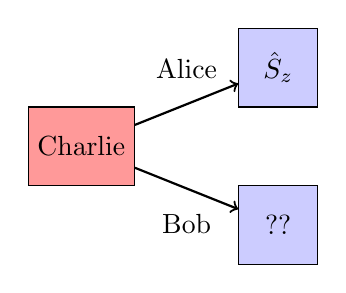
\begin{tikzpicture}
\node[fill=red!40,shape=rectangle,draw,minimum size=1cm](S) at (-0.5,0){Charlie};
\node[fill=blue!20,shape=rectangle,draw,minimum size=1cm](SG1) at (2,1){$\hat{S}_z$};
\draw[->,thick] (S) -- (SG1)node[midway,above,shift={(0,.2)}]{Alice};
\node[fill=blue!20,shape=rectangle,draw,minimum size=1cm](SG2) at (2,-1){??};
\draw[->,thick] (S) -- (SG2)node[midway,below,shift={(0,-.2)}]{Bob};
\end{tikzpicture}
\end{figure}

\sol The average measurement is then\arnote{Work through all the matrix multiplication here.}
\bas
\avg{\hat{S}_z} \Meq  &\Tr \begin{pmatrix}\frac{1}{3}&\frac{-\I\sqrt{2}}{3}\\\frac{\I\sqrt{2}}{3}&\frac{2}{3}\end{pmatrix}\frac{\hbar}{2}\szmatrix \\
&=\frac{\hbar}{2}\Tr \begin{pmatrix}\frac{1}{3}&\frac{\I\sqrt{2}}{3}\\\frac{\I\sqrt{2}}{3}&-\frac{2}{3}\end{pmatrix}\\
&=-\frac{\hbar}{6}.
\eas

We will also use the other method, just in case we hadn't realized that this was a product state. We first need the reduced density operator. We have the following coefficients:
\beq
\alpha_{uu} = \frac{1}{\sqrt{3}}\qquad \alpha_{du}=\I\sqrt{\frac{2}{3}}.
\eeq
The reduced density matrix, Eq.~(\ref{eq:reduceddensitymatrixcomp}) has four terms in it:
\bas
\rho_{uu} = & \alpha^{}_{uu}\alpha^*_{uu} + \alpha^{}_{ud}\alpha^*_{ud} = \frac{1}{3} \\
\rho_{ud} = & \alpha^{}_{uu}\alpha^*_{du} + \alpha^{}_{ud}\alpha^*_{dd} = -\I\frac{\sqrt{2}}{3} \\
\rho_{du} = & \alpha^{}_{du}\alpha^*_{uu} + \alpha^{}_{dd}\alpha^*_{ud} = \I\frac{\sqrt{2}}{3} \\
\rho_{dd} = & \alpha^{}_{du}\alpha^*_{du} + \alpha^{}_{dd}\alpha^*_{dd} = \frac{2}{3}.
\eas
Now we use Eq.~(\ref{eq:densitymatrixavgelements}) and add up the product of the components:\marginnote{There are only two non-zero components in $\hat{S}_z$: the $uu$ and the $dd$ components.}
\beq
\avg{\hat{S}_z} = \frac{\hbar}{2}\left(\rho_{uu} - \rho_{dd}\right) = -\frac{\hbar}{6}
\eeq

Finally we check her reduced density operator: it has only one eigenvalue of $1$, which is what we expect.

\assess We got the same answer both ways. Good.

\end{example}

\begin{exercise}
Alice and Bob start with combined ElMaW polarization state 
\beq
\ket{\Psi} = \frac{1}{\sqrt{2}}\left(\ket{VV} + \ket{HH}\right).
\eeq
What does Bob expect to get if he measures the average of the $V-H$ polarization of his component of the state?
\end{exercise}

\subsection{Decoherence and Measurement}
We previously described the process of decoherence where we lose phase information and thus the coherences of the density matrix go to zero. We now look at what happens to Alice's density matrix if Bob makes a measurement on his piece of the combined state. We'll start with the case where the combined state is a product state. In this case the reduced density matrix Eq.~(\ref{eq:reduceddensitymatrixcomp}) becomes
\bas
\rho_{aa'} = & \sum_b\bra{ab}\left(\oprod{A}{A}\otimes\oprod{B}{B}\right)\ket{a'b} \\
 = & \bra{a}(\oprod{A}{A})\ket{a'}\otimes \sum_b\bra{b}\oprod{B}{B}\ket{b} \\
 = & \bra{a}(\oprod{A}{A})\ket{a'},
\eas
which means that the reduced density operator is just the density operator composed of Alice's states: $\hat{\rho}_\rmt{Alice} = \oprod{A}{A}$.

Now what if the initial state was a pure state, but it wasn't a product state? Then what happens? Again we have
\beq
\rho_{aa'} =  \bra{a}\hat{\rho}\ket{a'} = \sum_b\alpha^{}_{ab}\alpha^*_{a'b}\;.
\eeq
So to write the density operator that gives rise to these matrix elements, we have the reduced density operator
\beq
\hat{\rho}_\rmt{Alice} = \sum_{jj',b} \alpha^{}_{jb}\alpha^*_{j'b} \oprod{j}{j'}.
\eeq\arnote[-1cm]{Check to make sure that this gives the proper density matrix elements.}
So what started out as a pure state has now become a mixed state. Alice has lost the phase information of the original state and is reduced to measuring probabilities. This means that measuring one piece of an entangled state has the same effect as losing coherence.

\begin{example}
Alice and Bob start with the entangled singlet state of atomic spins. Bob measures his state, but doesn't tell Alice anything. What now is Alice's density matrix?

\model We will work in the $z$-basis for both Alice and Bob and look at the matrix elements. We will model Alice's knowledge of the state as a reduced density matrix. We'll model the initial pure state as
\beq
\ket{\Psi} = \frac{1}{\stwo}\left(\ket{ud}-\ket{du}\right).
\eeq

\vis We have an entangled state that we've separated out.

\sol We figure out what Alice's density matrix elements are:\arnote{Work all of these out on your own.}
\bas
\rho_{uu} = & \alpha^{}_{uu}\alpha^*_{uu} + \alpha^{}_{ud}\alpha^*_{ud} = \frac{1}{2} \\
\rho_{ud} = & \alpha^{}_{uu}\alpha^*_{du} + \alpha^{}_{ud}\alpha^*_{dd} = 0 \\
\rho_{du} = & \alpha^{}_{du}\alpha^*_{uu} + \alpha^{}_{dd}\alpha^*_{ud} = 0 \\
\rho_{dd} = & \alpha^{}_{du}\alpha^*_{du} + \alpha^{}_{dd}\alpha^*_{dd} = \frac{1}{2}.
\eas

\assess As expected, Alice has lost all off-diagonal information and is left with a mixed state:
\beq
\hat{\rho} = \frac{1}{2}\oprod{u}{u} + \frac{1}{2}\oprod{d}{d}.
\eeq
She has a 50\% chance of measuring $\ket{u}$ and a 50\% change of measuring $\ket{d}$.

Alice's reduced density operator has the property of being proportional to the unit matrix with equal populations. That is the sign of a maximally entangled state.

\end{example}

\begin{exercise}
Alice and Bob start with the combined ElMaW polarization state
\beq
\ket{\Psi} = \frac{\I}{2}\ket{D_RD_R} + \frac{\sqrt{3}}{2}\ket{D_LD_L}.
\eeq
Alice measures her state, but doesn't tell Bob anything. What now is Bob's density matrix? What are the states Bob could measure and with what probabilities?
\end{exercise}

\section{Entanglement and Locality}
Is there any way that Alice and Bob, who share an entangled state, could use it to communicate? We've seen that they share a correlated measurement. Alice measures her state and it is correlated with Bob's state even if they are separated by a great distance. If we define a {\em local} interaction as one that does not permit information to move faster than the speed of light, we want to know if Alice and Bob can violate this.

Although Alice and Bob share an entangled state, we've seen that all Alice knows about is her reduced density matrix elements
\beq
\rho_{aa'} =  \bra{a}\hat{\rho}\ket{a'} = \sum_b\alpha^{}_{ab}\alpha^*_{a'b}.
\eeq
Can Bob do anything to change this, thus affecting Alice's measurements? We will limit Bob to unitary transformations on his part of the system, modeled as a unitary operator $\hat{U}$. For example, he could put his atomic spin in a uniform magnetic field and rotate it around. We model this unitary operator as a matrix with elements
\beq
U_{b'b} = \bra{b'}\hat{U}\ket{b}.
\eeq
So the initial combined state $\ket{\Psi}$ becomes
\bas
\ket{\Psi}_f = & \sum_{ab}\alpha_{ab}\hat{U}\ket{ab}=\sum_{ab} \alpha_{ab} \left(\onehat\otimes\hat{U}\right)\left(\ket{a}\otimes\ket{b}\right) \\
=& \sum_{ab} \alpha_{ab}\ket{a} \otimes\left(\hat{U}\ket{b}\right) \\
=& \sum_{ab}\alpha_{ab}\ket{a} \otimes\sum_{b'}\ket{b'}\bra{b'}\left(\hat{U}\ket{b}\right) = \sum_{ab,b'} \alpha_{ab}U_{b'b}\ket{ab'}.
\eas\marginnote[-1cm]{Using \ref{tool:span}}%
We rewrite this now, defining a new complex number that describes the amplitude of the state $\ket{ab'}$. The final state is thus
\beq
\ket{\Psi}_f = \sum_{ab'} \tilde{\alpha}_{ab'}\ket{ab'} \rmt{ with } \tilde{\alpha}_{ab'} = \sum_b \alpha_{ab}U_{b'b}.
\eeq
The bra-vector version of this is\arnote{Work this one out on your own using the bra-vector version.}
\beq
\bra{\Psi}_f = \sum_{a'b''} \tilde{\alpha}^*_{a'b''}\bra{a'b''} \rmt{ where }\tilde{\alpha}^*_{a'b''} = \sum_b \alpha^*_{a'b}U^\dagger_{bb''}.
\eeq
We can now find the matrix elements of Alice's final reduced density matrix:\marginnote{Note that we swapped the $b$ and $b'$ indices, as well as the $b$ and $b''$ indices. Since the notation is arbitrary, we can do this as long as we keep the ordering the same.}
\bas
\rho_{aa'} = & \sum_b\tilde{\alpha}^{}_{ab}\tilde{\alpha}^*_{a'b}= \sum_b \sum_{b'} \alpha_{ab'}U_{bb'} \sum_{b''} \alpha^*_{a'b}U^\dagger_{b''b} \\
=&  \sum_{bb'b''} \alpha^{}_{ab'} U^{}_{bb'}  U^\dagger_{b''b} \alpha^*_{a'b''}
\eas
but $U^{}_{bb'}  U^\dagger_{b''b} = \delta_{b'b''}$ so the reduced density matrix is
\beq
\rho_{aa'} = \sum_b\alpha^{}_{ab}\alpha^*_{a'b}
\eeq
and no change has happened. So there is nothing that Bob can do to change any of Alice's measurement outcomes. Locality is still intact.


\section{Bell Inequality Entanglement Test}
\marginnote{We are following Preskill's notes here.}We return now to correlations and joint measurements. We are again going to give Alice and Bob a combined state that they can each measure individually. We will measure four different sets of composite measurements and add them up in a clever way. Alice measures her states in two differnt basis: either the $\sigma_A$ or the $\sigma_{A'}$. Similarly, Bob measures either $\sigma_{B}$ or $\sigma_{B'}$ both of which can range from $+1$ to $-1$. We add up the four joint correlations as:
\beq
C\equiv\sigma_{A}\sigma_{B} + \sigma_{A'}\sigma_{B} + \sigma_{A}\sigma_{B'}-\sigma_{A'}\sigma_{B'}.
\eeq
Classically, if these states are independent we can factor these out to get
\beq
C=(\sigma_{A}+\sigma_{A'})\sigma_{B} + (\sigma_{A}-\sigma_{A'})\sigma_{B'}.
\eeq
Since both of these measurements range from $+1$ to $-1$, the largest that $(\sigma_{A}+\sigma_{A'})$ can be is $2$. However if it is $2$, then  $(\sigma_{A}-\sigma_{A'})=0$ and the other way around: if $(\sigma_{A}+\sigma_{A'})=-2$ the other is $0$. So that says that
\beq
\abs{C}\leq2. \rmt{ But that also means that } \abs{\avg{C}} \leq 2.
\eeq
In terms of the average measurements, that implies that 
\beq
\avg{\sigma_{A}\sigma_{B}} + \avg{\sigma_{A'}\sigma_{B}} + \avg{\sigma_{A}\sigma_{B'}}-\avg{\sigma_{A'}\sigma_{B'}} \leq 2.
\eeq
This is one version of the Bell Inequality. If any set of states do not obey this inequality, they must have some non-local correlation and are thus entangled.

\begin{example}
\label{ex:bell}
What is $C$ if Alice and Bob both start with the entangled polarization state
\beq
\ket{\Psi} = \frac{1}{\stwo}\left(\ket{VV} + \ket{HH}\right)
\eeq
and they make their measurements in the $V-H$ basis where the states are rotated before measurement with
\bas
\sigma_{A} \rightarrow & \rmt { rotate }90^\circ \rmt{ then measure }\hat{\sigma}_3 \\
\sigma_{A'} \rightarrow & \rmt{ measure }\hat{\sigma}_3 \\
\sigma_{B} \rightarrow & \rmt { rotate }45^\circ \rmt{ then measure }\hat{\tau}_3 \\
\sigma_{B'} \rightarrow & \rmt { rotate }135^\circ \rmt{ then measure }\hat{\tau}_3
\eas

\model We will model \hwp the rotations using a unitary operators using matrix notation in the $V-H$ basis where
\beq
\hat{U}(\theta) \Meq  \begin{pmatrix}\cos\theta&\sin\theta\\-\sin\theta&\cos\theta\end{pmatrix}
\eeq

This means that the combined rotations and measurements do the following:\arnote{Use the rotation matrix and the $\hat{\sigma}_3$ operator to evaluate these.}
\bas
\hat{\sigma}_{A}\ket{V} = &  \ket{H} & \hat{\sigma}_{A}\ket{H} = &  \ket{V} \\
\hat{\sigma}_{A'}\ket{V} = &  \ket{V} & \hat{\sigma}_{A'}\ket{H} = &  -\ket{H} \\
\hat{\tau}_{B}\ket{V} = &  \frac{1}{\stwo}(\ket{V}+\ket{H}) & \hat{\tau}_{B}\ket{H} = &  \frac{1}{\stwo}(\ket{V}-\ket{H})\\
\hat{\tau}_{B'}\ket{V} = &  \frac{1}{\stwo}({-\ket{V}}+\ket{H}) & \hat{\tau}_{B'}\ket{H} = &  \frac{1}{\stwo}(\ket{V}+\ket{H})
\eas

\vis We've got a very similar situation as before, but now Alice and Bob could make one of two measurements. They will get together later to combine their results and calculate the correlations.

\begin{figure}
\centering
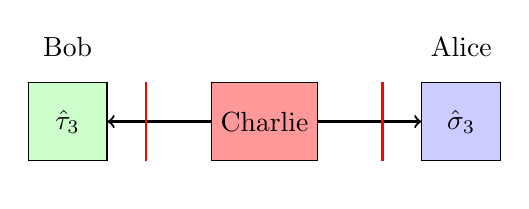
\begin{tikzpicture}
\node[fill=red!40,shape=rectangle,draw,minimum size=1cm](S) at (-0.5,0){Charlie};
\node[fill=blue!20,shape=rectangle,draw,minimum size=1cm](SG1) at (2,0){$\hat{\sigma}_3$};
\draw[->,thick] (S) -- (SG1)node[right,above,shift={(0,.7)}]{Alice};
\draw[red,thick] (1,-.5)node[below,black]{\hwp} -- (1,.5);
\node[fill=green!20,shape=rectangle,draw,minimum size=1cm](SG1b) at (-3,0){$\hat{\tau}_3$};
\draw[->,thick] (S) -- (SG1b)node[left,above,shift={(0,.7)}]{Bob};
\draw[red,thick] (-2,-.5)node[below,black]{\hwp} -- (-2,.5);
\end{tikzpicture}
\end{figure}

\sol This takes a bit of work, but we use our tensor product tools to find that
\bas
\avg{\hat{\sigma}_{A}\hat{\tau}_{B}} & = \frac{1}{\stwo} \\
\avg{\hat{\sigma}_{A'}\hat{\tau}_{B}} & = \frac{1}{\stwo}\\
\avg{\hat{\sigma}_{A}\hat{\tau}_{B'}} & = \frac{1}{\stwo}\\
\avg{\hat{\sigma}_{A'}\hat{\tau}_{B'}} & = -\frac{1}{\stwo}
\eas
So the sum total is
\beq
C = 2\sqrt{2} > 2
\eeq
and the inequality is violated.

\assess The state we started with is maximally entangled, so we expected something non-classical for the result. This is actually the largest violation possible for our quantum mechanical model.

\end{example}

\begin{exercise}
What is $C$ if Alice and Bob both start with the polarization state
\beq
\ket{\Psi} = \frac{1}{\sqrt{3}}\ket{VV} + \I\sqrt{\frac{2}{3}} \ket{VH}
\eeq
and measure using the same plan as in Example~\ref{ex:bell}?

\end{exercise}

\begin{exercise}
What is $C$ if Alice and Bob both start with the polarization state
\beq
\ket{\Psi} = \frac{1}{3}\ket{VV} + \I\frac{1}{3} \ket{VH} + \frac{\sqrt{7}}{3} \ket{HH}
\eeq
and measure using the same plan as in Example~\ref{ex:bell}?

\end{exercise}

%http://www.theory.caltech.edu/~preskill/ph229/notes/chap4_01.pdf
%http://research.physics.illinois.edu/QI/Photonics/papers/My%20Collection.Data/PDF/The%20mystery%20of%20the%20quantum%20cakes.pdf

\section{Entanglement and Measurement Instruments}
\begin{marginfigure}
\begin{tikzpicture}[scale=0.6]
\draw (-0.5,-.5) rectangle +(1,1);
\draw (-.5,-.5) -- (.5,.5);
\draw[red,->,decorate, decoration={snake,amplitude=5,segment length=10, post length=.1cm}](-3.3,0)--(-.55,0) node[midway, above,shift=({0,.2cm})]{};
\draw[red,->,decorate, decoration={snake,amplitude=5,segment length=10, post length=.1cm}](.55,0)--(2,0);
\detector{1}{2.1}{0}{0}
\node at (3,-1) {Detector 1};

\draw[red,->,decorate, decoration={snake,amplitude=5,segment length=10, post length=.1cm}](0,.55)--(0,2);
\detector{1}{0}{2.1}{90}
\node at (2,2.5) {Detector 2};

\draw[thick,green] (-2.5,-1) -- (-2.5,1);
\draw[thick,blue] (-1.5,-1) -- (-1.5,1) ;
\fill[black,opacity=0.3](-3,-1.2) rectangle (1.4,1.4) node[midway,below,black,opacity=1,shift={(0,-0.7)}]{Operator Model};


\begin{scope}[shift={(-3,-4)},scale=1.3]

%atom beam
\fill[color=green!80,thick,decorate, decoration={shape backgrounds, shape=circle,shape size=0.2cm,shape sep={0.4cm, between centers}}](0,0,0) -- (2.4,0,0) ;

\begin{scope}[shift={(2.4,0,0)}]
\fill[color=green!80,thick,decorate, decoration={shape backgrounds, shape=circle,shape size=0.1cm,shape sep={0.4cm, between centers}}](0,0) -- (20:3.0);
\fill[color=green!80,thick,decorate, decoration={shape backgrounds, shape=circle,shape size=0.1cm,shape sep={0.4cm, between centers}}](0,0) -- (-20:3.0);
\end{scope}

%field gradient zone
\begin{scope}[shift={(0,.15,0)}]
\begin{scope}[canvas is xz plane at y=.5,shift={(2,0,0)}]
\fill[blue,opacity=0.5] (-.5,-.5) rectangle +(1,1);
\end{scope}
\begin{scope}[canvas is yz plane at x=2.5]
\fill[blue,opacity=0.4] (-.5,-.5) rectangle +(1,1);

\end{scope}
\begin{scope}[canvas is xy plane at z=.5,shift={(2,0,0)}]
\fill[blue,opacity=0.3] (-.5,-.5) rectangle +(1,1);

\end{scope}

\draw[->,thick](2.5,-.5,-.5)--(2.5,.5,-.5);

\end{scope}


\begin{scope}[canvas is yz plane at x=5]
\fill[orange,opacity=0.4] (-1,-1) rectangle +(2,2);
\end{scope}
%\node[text width=2cm,align=center] at (4.5,-1.1,0) {Atom Position Detector};

\fill[black,opacity=0.3](1,-1) rectangle (3,1)node[midway,below,black,opacity=1,shift={(0,-0.7)}]{Operator Model};


\end{scope}

\end{tikzpicture}
\end{marginfigure}
We are at a point where we can build a model to describe what happens to the quantum state between the operator model and the actual measurement apparatus. In Section~\ref{sec:operatormodel4} we modeled the physical interaction zones as linear operators. We now model what happens between that model and the moment the detectors register either a photoelectron (in the ElMaW case) or the detectors register an atom (in the spin case). We'll focus on the ElMaW detectors and model them as a quantum system in one of the following states:
\beq
\rmt{``blank''}\rightarrow\ket{b}\quad\rmt{``V measured''}\rightarrow \ket{+1} \quad\rmt{``H measured''}\rightarrow \ket{-1}.
\eeq
So the combined state of both the ElMaW and the detectors has six possible states. In the moment after the ElMaW has passed through the beamsplitter but before it reaches the detectors, the combined state is a product state (writing this as $\ket{\rmt{ElMaW},\rmt{Dectector}}$)
\beq
\alpha_V \ket{V,b} + \alpha_H\ket{H,b}.
\eeq
We know what happens to this state when the detectors register a photoelectron. A $V$ registers as a $+1$ an $H$ registers as a $-1$. So after the ElMaW interacts with the detectors, we have the maximally entangled state
\beq
\alpha_V \ket{V,+1} + \alpha_H\ket{H,-1}.
\eeq
Now whether we say that the detector's quantum state is uncontrolled and thus is subject to rapid decoherence, or if we say we only have access to the ElMaW piece of the state and thus we need to look at the reduced density operator, we get the same result. The state we have access to reduces from a quantum system to a mixed state. We are left with classical probabilities. This model of detector-entanglement measurement works reasonably well for a number of situations. 


\chapter{Continuous Quantum States}

We now move to another type of quantum system. Up until now we have focused on the ElMaW polarization quantum states and the atomic spin quantum states. But there are other situations where our classical point particle model fails to describe the behavior of the system. There are experiments where electrons, atoms, and molecules exhibit behavior that is not consistent with the point particle model. In these experiments, we are interested in the position and the momentum of the system, so we need to develop a quantum model for working with these new, continuous parameters for describing our quantum state.

\section{Wavefunctions}

We previously used a set of basis states $\ket{\lambda}$ that were eigenvectors of an operator to decompose any arbitrary quantum state:
\beq
\ket{\Psi} = \sum_\lambda \alpha_\lambda \ket{\lambda}.
\eeq\marginnote[-1cm]{\ref{tool:decom}}
We now extend this model to include the possibility of the eigenvectors and the eigenvalues being {\em continuous}, instead of discrete states. Since the eigenvectors are continuous, we need to describe the components $\alpha_\lambda$ in terms of a continuous function instead of discrete complex values. We define this new parameter as $\psi(\lambda)$, a complex-valued function of $\lambda$.\marginnote[-1cm]{Recall that we previously saw that complex-valued functions behave like vector spaces themselves!}

The quantum state is now decomposed in terms of these new, continuous basis functions:
\beq
\ket{\Psi} = \sum_\lambda \psi(\lambda)\ket{\lambda}
\eeq\marginnote[-1cm]{\ref{tool:orthog}}%
where
\beq
\psi(\lambda) = \avg{\lambda|\Psi}.
\label{eq:wavefunction}
\eeq\toolnote[-0.7cm]{\toollabel{tool:wavefunction}{\includegraphics{tool11.tikz} {\bf Wavefunctioner}}.  This tool is used to determine the continuous wavefunction in a particular basis.} 
These amplitudes $\psi(\lambda)$ are called {\em wavefunctions} and describe the quantum state $\ket{\Psi}$ in the $\lambda$ basis. As we previously saw with CSCOs, there may be more than one set of basis states needed to uniquely describe our quantum system. In that case, the wavefunction becomes a multi-variable complex-valued function of all the basis states $\psi(\lambda, \delta, \gamma, \ldots)$.


\section{Position Basis}

We begin working with continuous quantum states by looking at the position basis. We want to model the behavior of a single electron confined to move in a single dimension. This is a crude model of the position of an electron in a beam or the position of an electron in a very long, thin wire. We will work in the $\ket{x}$ basis where $\ket{x}$ describes the quantum position eigenvectors of our system. In this basis, our wavefunction is 
\beq
\psi(x) = \avg{x|\Psi} \rmt{ and }\psi^*(x) = \avg{\Psi|x}.
\label{eq:defwavefunction}
\eeq\marginnote[-1cm]{\ref{tool:wavefunction}.}%
Because the position eigenvectors are continuous -- they could be any real value along the one dimension of travel -- we need to adapt our tools to work with continuous variables. The first change is that discrete sums become integrals:
\beq
\sum_i \rightarrow \int dx
\eeq
So our \ref{tool:span} becomes
\beq
\intii \ket{x}\bra{x} dx = \onehat.
\eeq\marginnote[-1cm]{Since we are now dealing with position, our basis vectors $\ket{x}$ now have units. In order to make this work, they have to have units [1/$\sqrt{\rmt{length}}$].} We want to use this to develop a continuous version of the inner product and probability projection. Before we do that, though, we need a new math tool.

\subsection{The Dirac Delta}
We take a quick side trip to define the {\em Dirac delta functional}. It is not mathematically a function, but it is often called that. Recall that we used the Kronecker delta to collapse sums of discrete states:
\beq
\sum_j \delta_{jk}A_k = A_j.
\eeq
The Dirac delta does a similar thing with continuous integrals. It is defined as the thing that makes
\beq
\intii \delta(x-x')F(x')dx' = F(x)
\label{eq:diracdelta}
\eeq\marginnote[-1cm]{The $\delta(x)$ functional also has units to make this work. Its units are [1/length].}
work. In effect, it is zero everywhere except at one point $x$ where it is, in effect, infinite. It can be approximated with a lot of real functions -- a Gaussian function $(n/\sqrt{\pi})\E{-(nx)^2}$ does a good job of making this work as $n\rightarrow \infty$. \begin{marginfigure}
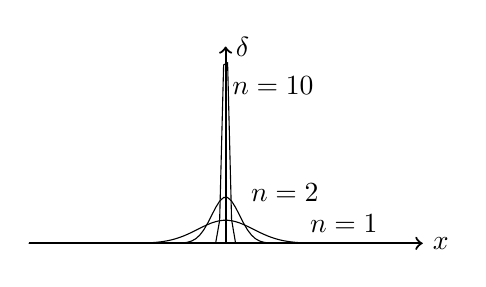
\begin{tikzpicture}[scale=0.5]
\draw[->,thick] (-5,0) -- (5,0) node[right]{$x$};
\draw[->,thick] (0,0) -- (0,5) node[right]{$\delta$};

\foreach \n in {1,2,10}
\draw[domain=-5:5,samples=100] plot({\x},{\n/1.7*exp(-(\n*\x)^2});

\node at (3,.5) {$n=1$};
\node at (1.5,1.3) {$n=2$};
\node at (1.2,4) {$n=10$};

\end{tikzpicture}
\end{marginfigure}
The function $F(x')$ could be a constant in which case
\beq
\intii \delta(x-x')dx' = 1.
\eeq

\begin{exercise}
Show that the Gaussian approximation for the Dirac Delta function satisfies Eq.~(\ref{eq:diracdelta}) for $F(x) = x^2$ and $F(x) = x^3$. What is the difference between the model and the actual result in terms of $n$?
\end{exercise}

%\begin{exercise}
%Evaluate the following integrals using the properties of the Dirac delta function.
%\bas
%\rmt{(a) }&  \int^{\infty}_{-\infty}\,\delta(x)\cos(x) dx &   \rmt{(b) }& \int^{\infty}_{0}\,\delta(x+\pi)\cos(x) dx \\
%\rmt{(c) }& \int^{\infty}_{0}\,\delta(x-2)\, x^{2}dx &  \rmt{(d) }&  \int^{1/2}_{-1/2}\,\delta(x)\, (x - 3)dx \\
%\rmt{(e) }& \int^{3}_{2}\,\delta(x+2)\, (x - 2)dx & 
%\eas
%\end{exercise}

\subsection{Back to Continuous States}

We now define the inner product for continuous basis functions. Previously we had
\beq
\avg{j|k} = \delta_{jk}.
\eeq
We get the continuous version of this starting with the action of the $\onehat$ operator which we want to leave the state unchanged: $\onehat\ket{x'} = \ket{x'}$. We insert the continuous spanner tool on the left side:
\beq
\onehat\ket{x'} =  \intii \left(\ket{x}\bra{x}\right)\ket{x'}dx =\intii \ket{x}\avg{x|x'}dx = \ket{x'}.
\eeq
So that means that $\avg{x|x'} = \delta(x-x')$.

We now use this to define the general inner product between two quantum states in terms of the wavefunctions in the position basis. \marginnote[1cm]{Using \ref{tool:span} twice.}
\bas
\avg{\Psi|\Phi} = & \iint\displaylimits_{-\infty}^\infty \avg{\Psi|x^{}}\bra{x^{}}\ket{x'}\avg{x'|\Phi}dx dx'\\
= & \iint\displaylimits_{-\infty}^\infty \avg{\Psi|x^{}}\delta(x-x')\avg{x'|\Phi}dx dx' \\
= & \intii \avg{\Psi|x}\avg{x|\Phi}dx \\
= & \intii \psi^{*}(x)\phi^{}(x)dx 
\eas\marginnote[-1cm]{\ref{tool:wavefunction}.}%
where we used the definition of the wavefunction, Eq.~(\ref{eq:defwavefunction}), to write the inner product in terms of the wavefunctions in the position basis. Since our quantum states are normalized, the inner product of a quantum state with itself is one:
\beq
\intii \psi^{*}(x)\psi^{}(x)dx = 1.
\label{eq:normwavefunction}
\eeq  \marginnote{This means that the wavefunction in the position basis also has units [1/$\sqrt{\rmt{length}}$].} In order for our quantum state to be normalizable we must be able to integrate along the entire one-dimensional space and get a finite, unit answer. That puts limits on what we can use for our wavefunctions in the position basis. They must be {\em square integrable} since the integral of the wavefunction times its complex conjugate must be one.

\section{Measurement Probabilities}

We previously connected the amplitudes $\alpha_k$ with the probability of measuring a state with eigenvector $\ket{k}$: $P(\ket{k}) = \abs{\avg{k|\Psi}}^2$.\marginnote{\ref{tool:prob}} We do the same thing with the wavefunctions in the position basis. But we now need to specify the region over which we are interested in finding the probability. So if we want to know what the probability is that the quantum state lies between the points $a$ and $b$, we look at
\beq
P(a,b) = \int\displaylimits_a^b\psi^{*}(x)\psi^{}(x)dx.
\eeq\marginnote[-1cm]{This updates the \ref{tool:prob}.}%
This connects nicely with our continuous normalization Eq.~(\ref{eq:normwavefunction}) which we can now say that this means that there is a 100\% change of measuring the system somewhere along the infinite line. \marginnote{The probability density has units [1/length].} This means that the product $\Pd(x) \equiv \psi^{*}(x)\psi^{}(x)$ is not a probability, but a {\em probability density}. This is slightly different from the discrete case where $\abs{\alpha_k}^2$ was the probability of measuring the state $\ket{k}$. With this notation, the probability of finding the state in the interval $(a,b)$ is
\beq
P(a,b) = \int\displaylimits_a^b\Pd(x)dx \rmt{ and } \intii \Pd(x)dx = 1.
\eeq

\begin{example}
\label{ex:oneDwirePD}
An electron is confined to a long, thin wire. What is the probability density if the electron could be anywhere along the wire with equal probability?

\model We are going to model the electron as a 1-D continuous quantum system along the $x$-axis. We will work in the $x$-basis. We model the wire as having length $L$ centered on $x=0$.

\vis Our system looks something like Figure~\ref{fig:ex191}
\begin{figure}
\centering
\begin{tikzpicture}
\node[name=A,cylinder,draw=black,thick,minimum height=6cm,minimum width=0.3cm,cylinder uses custom fill, cylinder body fill=black!20,cylinder end fill=black!30] at (0,0) {};
\draw[->,thick] (-4,0) -- (4,0) node[right]{$x$};
\draw[->,thick] (0,-2) -- (0,2) node[right]{$y$};
\draw[-] (3,-.5) -- (3,-1)node[below]{$x=L/2$};
\draw[-] (-3,-.5) -- (-3,-1)node[below]{$x=-L/2$};
\end{tikzpicture}
\caption[][2cm]{ }
\label{fig:ex191}
\end{figure}

\sol In our model the electron can only be somewhere between $-L/2$ and $L/2$. So we want the probability of finding the electron to be one along this length. Since the probability density is constant, let's call it $\Pd$ and find the normalization:
\beq
\avg{\Psi|\Psi} = \int\displaylimits_{-\infty}^{\infty}\Pd dx = 1.
\eeq
We need a probability density that is zero everywhere expect from $-L/2$ to $L/2$. So the integral becomes
\beq
\int\displaylimits_{-L/2}^{L/2}\Pd dx = L\Pd.
\eeq
That means that the probability density is \arnote{Fill in the skipped steps here.}
\beq
\Pd(x) = \begin{cases}1/L &\rmt{ if } -L/2\leq x \leq L/2, \\ 0 &\rmt{otherwise}.\end{cases}
\eeq

\assess Our probability density has units 1/length as expected.

\end{example}

\begin{exercise}
An electron is confined to a long, thin wire. What is the (complex-valued) wavefunction in the position basis if the electron could be anywhere along the wire with equal probability?
\end{exercise}

Suppose we measured the state in the interval $(a,b)$. What is the state after we've made this measurement? We don't know much more than the state is in this interval and that the state must still be normalized. However, the normalization must have changed because the probability of finding the state in this interval after the measurement must be $1$:
\beq
P_\rmt{after}(a,b) = \int\displaylimits_a^b\Pd_\rmt{after}(x)dx=1.
\eeq%
In order to make this happen, we need to {\em renormalize} the wavefunction. This means we set an arbitrary constant in front of the wavefunction and apply the normalization condition to find the new wavefunction.

\begin{example}
\label{ex:electronwire}
An electron is confined to a long, thin wire with uniform probability density. What is the probability of measuring the position of the electron in the region $0\leq x \leq L/4$? What is the state after the measurement?

\model We model the electron as a 1D quantum state in the position basis, confined to a wire of length $L$. Our probability density was found in Example \ref{ex:oneDwirePD}.

\vis We are interested in the red zone in Figure~\ref{fig:ex192}.
\begin{figure}
\centering
\begin{tikzpicture}
\node[name=A,cylinder,draw=black,thick,minimum height=6cm,minimum width=0.3cm,cylinder uses custom fill, cylinder body fill=black!20,cylinder end fill=black!30] at (0,0) {};
\draw[->,thick] (-4,0) -- (4,0) node[right]{$x$};
\draw[->,thick] (0,-2) -- (0,2) node[right]{$y$};
\draw[-] (3,-.5) -- (3,-1)node[below]{$x=L/2$};
\draw[-] (-3,-.5) -- (-3,-1)node[below]{$x=-L/2$};
\node[rectangle,minimum width=1.5cm,minimum height=0.6cm,opacity=0.4,fill=red] at (0.75,0){};
\end{tikzpicture}
\caption[][2cm]{ }
\label{fig:ex192}
\end{figure}

\sol The probability of finding the electron is modeled as\arnote[1cm]{Fill in the missing steps here, too.}
\bas
P(0\leq x\leq L/4) = & \int_0^{L/4}\Pd(x)dx \\
=& \frac{1}{L}\left( \frac{L}{4} \right) = \frac{1}{4}.
\eas
After the measurement, we know that the electron must be in the interval from $0\leq x\leq L/4$, so we renormalize the wavefunction using an arbitrary constant $A$:
\bas
P(0\leq x\leq L/4)= 1 = & \int_0^{L/4}\abs{A}^2\Pd(x)dx \\
=&\frac{\abs{A}^2}{4}
\eas
so the new normalized wavefunction is $\ket{\psi} = 2/\sqrt{L}$ over the interval $0\leq x\leq L/4$ and zero everywhere else.

\assess Since the probability density was uniform and we're looking at a quarter of the length of the wire, we expect the probability to be 25\% as we found.

\end{example}

\section{Continuous Operators}

The next piece is to define the action of linear operators in our continuous basis space. We are interested in the average measurement of the operator in the position basis. \marginnote[1cm]{\ref{tool:avg}
\ref{tool:span}}
\bas
\avg{\hat{M}} & = \bra{\Psi}\hat{M}\ket{\Psi} \\
& = \iint\displaylimits_{-\infty}^\infty \avg{\Psi|x}\bra{x}\hat{M}\ket{x'}\avg{x'|\Psi}dx dx'\\
& = \iint\displaylimits_{-\infty}^\infty \psi^{*}(x)\bra{x}\hat{M}\ket{x'}\psi^{}(x')dx dx'
\eas
We need to know more about the operator in the $\bra{x}\hat{M}\ket{x'}$ basis before we can evaluate this.

\subsection{The Position Operator}
The position operator $\hat{X}$\marginnote{Note the use of the upper-case $X$ in the operator. Don't confuse this with the 3-vector unit vector $\hat{x}$.} is the Hermitian operator for which our position vectors $\ket{x}$ are eigenvectors with eigenvalues $x$:
\beq
\hat{X}\ket{x} = x\ket{x}.
\eeq
If we want to find the portion of a quantum state at $\ket{x_0}$, we should be able to find $\avg{x_0|\Psi}$. We know that $\avg{x|x_0} = \delta(x-x_0)$. So we have \marginnote[1cm]{\ref{tool:span}}
\bas
\avg{x_0|\Psi} = & \int\displaylimits_{-\infty}^{\infty} \avg{x_0|x}\avg{x|\Psi}dx \\
= & \int\displaylimits_{-\infty}^{\infty} \delta(x-x_0)\psi(x)dx  = \psi(x_0),
\eas\marginnote[-1cm]{\ref{tool:wavefunction}.}%
which is the general wavefunction evaluated at position $x_0$. This is what we want. We can now find the $\hat{X}$ operator in the $\ket{x}$ basis. \arnote{I've skipped steps here - fill them in in your notes.}
\marginnote[2cm]{\ref{tool:span}}%
\bas
\avg{\hat{X}} & = \bra{\Psi}\hat{X}\ket{\Psi} \\
& = \iint\displaylimits_{-\infty}^\infty \psi^{*}(x)\bra{x}\hat{X}\ket{x'}\psi^{}(x')dx dx'\\
& = \iint\displaylimits_{-\infty}^\infty \psi^{*}(x)x'\avg{x|x'}\psi^{}(x')dx dx'\\
& = \intii \psi^{*}(x)x\psi^{}(x)dx.
\eas
So the position operator in the $\ket{x}$ basis is
\beq
\bra{x}\hat{X}\ket{x'} = x'\delta(x-x')
\eeq
and we have a way of calculating the average position in the $\ket{x}$ basis. We can run the same procedure again and also get
\beq
\avg{\hat{X}^2} = \intii \psi^{*}(x)x^2\psi^{}(x)dx.
\eeq
With these two together we can calculate the uncertainty in the measurement of the average position as well, Eq.~(\ref{eq:uncert}).\marginnote{\ref{tool:meunc}}%

\begin{example}
What is the average position measurement with its uncertainty for the electron in Example \ref{ex:oneDwirePD}?

\model We'll model the electron as a 1-D quantum system confined to move along a 1-D wire of length $L$. We'll model the wavefunction as a uniform probability density with $\psi(x) = 1/\sqrt{L}$.

\vis Our system looks like Figure~\ref{fig:ex193}.
\begin{figure}
\centering
\begin{tikzpicture}
\node[name=A,cylinder,draw=black,thick,minimum height=6cm,minimum width=0.3cm,cylinder uses custom fill, cylinder body fill=black!20,cylinder end fill=black!30] at (0,0) {};
\draw[->,thick] (-4,0) -- (4,0) node[right]{$x$};
\draw[->,thick] (0,-1.5) -- (0,1) node[right]{$y$};
\draw[-] (3,-.25) -- (3,-.75)node[below]{$x=L/2$};
\draw[-] (-3,-.25) -- (-3,-.75)node[below]{$x=-L/2$};
\end{tikzpicture}
\caption[][2cm]{ }
\label{fig:ex193}
\end{figure}

\sol We want the average position in the $x$ basis:
\bas
\avg{\hat{X}} & = \bra{\Psi}\hat{X}\ket{\Psi} \\
& = \iint\displaylimits_{-\infty}^\infty \psi^{*}(x)\bra{x}\hat{X}\ket{x'}\psi^{}(x')dx dx' \\
& =  \frac{1}{L}\int\displaylimits_{-L/2}^{L/2}x dx \\
\avg{\hat{X}} & = \frac{1}{L} \left(\frac{L^2}{4} -\frac{L^2}{4}  \right) = 0.
\eas
\arnote[-2cm]{Of course I skipped steps here. Make sure you know what they are! Same thing with the other calculation.} So the average measurement of the position operator is $0$ which makes sense given the probability density function.

We also need
\bas
\avg{\hat{X}^2} & = \bra{\Psi}\hat{X}^2\ket{\Psi} \\
& = \iint\displaylimits_{-\infty}^\infty \psi^{*}(x)\bra{x^{}}\hat{X}^2\ket{x'}\psi^{}(x')dx dx' \\
& =  \frac{1}{L}\int\displaylimits_{-L/2}^{L/2}x^2 dx \\
\avg{\hat{X}^2} & = \frac{1}{3L} \left(\frac{L^3}{8} -\frac{-L^3}{8}  \right) = \frac{L^2}{12}.
\eas
So the uncertainty is $\Delta X = \sqrt{\avg{\hat{X}^2}}$ (since $\avg{\hat{X}}=0$) is\marginnote{\ref{tool:meunc}}%
\beq
\Delta X = \frac{L}{\sqrt{12}}.
\eeq

\assess Both of our answers make sense and have the correct units. The uncertainty of the position measurement is half the total length of the wire, which is interesting. That means that over time, many repeated measurements will have a wide uncertainty.

\end{example}


\begin{exercise}

Consider the probability density for finding an electron along a 1-D line:
%
\beq
\Pd(x) = A\left(\frac{x}{L}\right)^{2}\E{-x^{2}/L^{2}},
\eeq
%
where $A$ is a normalization constant and $L$ is a constant length scale.
\begin{enumerate}
\item[(a)]  Determine $A$ so the probability density is properly normalized.  What are the units of $A$?
\item[(b)]  Plot $\Pd(x)$.
\item[(c)]  Find the position(s) where the electron is most likely to be found, \ie where the probability density is greatest.  Then determine the position(s) where the electron is least likely to be found.
\item[(d)]  Determine the probability that the electron will be found in the region $0 \leq x \leq L$.
\item[(e)] What is the state of the electron if it was measured in the region $0 \leq x\leq L$? 
\end{enumerate}

\end{exercise}

\begin{exercise}
What are the average measurements of the position operator and its uncertainty for the probability distribution from the previous exercise?
\end{exercise}

\chapter{Momentum Eigenvectors}

So far we've built a model for describing the position of a quantum system. That is a good start, but that doesn't fully describe the state of many systems. For example, we could have two atoms, both in the same position, but with very different momenta. The position quantum state isn't sufficient to distinguish those two very different states. So let's build a model for describing the continuous quantum momentum.
\begin{marginfigure}[-2cm]
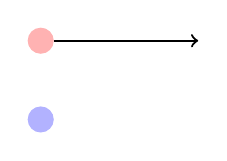
\begin{tikzpicture}[scale=2]
\node[circle, fill=blue!30] at (0,0){};
\node[circle, fill=red!30](A) at (0,.5){};
\draw[->, thick] (A) -- (1,.5);
\end{tikzpicture}
\end{marginfigure}

\section{Momentum Basis}
We repeat everything we did for the position basis $\ket{x}$, but this time expand our quantum state with the basis vectors $\ket{p_x}$. The formalism is all the same and we end up with very similar results. The momentum operator in the momentum basis is
\beq
\hat{P}_x \ket{p_x} = p_x\ket{p_x}.
\eeq
The orthogonality relationship is
\beq
\avg{p_x|p'_x} = \delta(p_x - p'_x).
\eeq\marginnote[-1cm]{This time the delta functional has units [1/momentum]. In general its units will be 1 over the units of the thing inside the parenthesis.}
The momentum operator in the momentum basis is
\beq
\bra{p_x}\hat{P}_x\ket{p'_x} = p_x \delta(p_x - p'_x).
\eeq
We can expand any state in terms of the complete, orthonormal momentum basis
\beq
\int\displaylimits_{-\infty}^{\infty}\ket{p_x}\bra{p_x}dp_x = \onehat.
\eeq
And the wavefunctions in the momentum basis are
\beq
\avg{p_x|\Psi} = \phi(p_x).
\eeq\marginnote[-2cm]{We've called these wavefunctions $\phi(p_x)$ instead of $\psi$ to help keep them different since they are a function of $p_x$, not a function of $x$. Note that $\phi(p_x)$ has units [1/$\sqrt{\rmt{momentum}}$]. We used \ref{tool:wavefunction} here, too.}%
So far, so good. But it is useful to write the momentum operator in the position basis and to be able to switch between bases. For example, we have an atom moving in one dimension. We know its position state at one moment in time but would like to know about its position at a future time point. We need to switch to the momentum basis, let the quantum state evolve with time, then switch back to the position basis and evaluate its position. We'll look at these tools next.

\begin{example}
An atom is moving with momentum wave function given by 
\beq
\phi(p_x) = A \E{-p_x^{2}/(2p_0^{2})},
\eeq
where $p_{0}$ and $A$ are constants. What is the average momentum measurement with its uncertainty for this atom?

\model We model the atom as a quantum system in the momentum basis moving in one dimension. 

\vis The momentum wavefunction looks like this:
\begin{figure}
\centering
\begin{tikzpicture}[scale=0.6]
\draw[->,thick] (-5,0) -- (5,0) node[right]{$p_x$};
\draw[->,thick] (0,0) -- (0,5) node[right]{$\phi$};

\draw[domain=-5:5,samples=100] plot({\x},{4*exp(-(\x)^2});

\end{tikzpicture}
\end{figure}

\sol We first need to normalize the wavefunction. We must have
\bas
1 = \avg{\Psi|\Psi} = & \int\displaylimits_{-\infty}^{\infty}\phi(p_x)^{*}\phi^{}(p_x)dp_x \\
= & \abs{A}^2\int\displaylimits_{-\infty}^{\infty} \E{-p_x^{2}/p_0^{2}} dp_x \\
= & \abs{A}^2 \sqrt{\pi} p_0.
\eas
That means that, in order to be normalized, $A = 1/\sqrt{\sqrt{\pi}p_0}$.

We now find the average measurement and uncertainty:
\bas
\avg{\hat{P}_x} =  & \frac{1}{\sqrt{\pi}p_0}\left[\int\displaylimits_{-\infty}^{\infty} p_x \E{-p_x^{2}/p_0^{2}} dp_x\right]^{1/2} \\
=& 0.
\eas
And we have
\bas
\Delta P_x = &\sqrt{\avg{\hat{P}_x^2}} \\
= & \frac{1}{\sqrt{\pi}p_0}\int\displaylimits_{-\infty}^{\infty} p_x^2 \E{-p_x^{2}/p_0^{2}} dp_x \\
=&\frac{p_0}{\sqrt{2}}.
\eas

\assess The units on $A$ are [1/$\sqrt{\rmt{momentum}}$] which is what we expect. The average and the uncertainty are also both as expected for a Gaussian distribution.

\end{example}

\begin{exercise}
An atom is moving in one dimension with a momentum wave function given by
%
\beq
\phi(p_{x}) = \frac{A}{1 + (p_{x}/p_{0} -1)^{2}}
\eeq
%
where $p_{0}$ and $A$ are constants.
\begin{enumerate}
\item[(a)] Find $A$ so the wave function is properly normalized.  What is the dimension of $A$?
\item[(b)]  Graph $\phi(p_{x})$.
\item[(c)]  Find the most probable value of momentum.
\item[(d)] Find the probability that the atom has momentum in the range $p_{0} \leq p_{x} \leq 2p_{0}$.
\item[(e)]  Suppose the particle's momentum is measured and found to be negative (i.e., in the range $-\infty \leq p_{x} \leq 0$).  Find the momentum wave function immediately after the measurement.

\end{enumerate}
\end{exercise}

\section{Momentum operator in the position basis}
\label{sec:momentuminposbasis}
We've looked at changing bases before when we switched between the $z$-basis and the $x$-basis describing our quantized spin states. We start with the momentum operator acting on a momentum eigenstate and then expand this in terms of the position basis.
\bas
\hat{P}_x \ket{p_x} & = p_x\ket{p_x}\\
\bra{x}\hat{P}_x \ket{p_x} & = p_x\avg{x|p_x}\\
\int\displaylimits_{-\infty}^{\infty}\bra{x}\hat{P}_x\ket{x'} \avg{x'|p_x} dx'& = p_x\avg{x|p_x} \label{eq:momentumexpansion}
\eas
As before, we need to know what the matrix elements of the momentum operator in the position basis are. We'll try one and then show that it has the properties that we want. The momentum operator in the position basis is a differential operator
\beq
\bra{x}\hat{P}_x\ket{x'} \equiv -\I\hbar \delta(x-x')\frac{\partial}{\partial x'}.
\label{eq:momentummatrix}
\eeq \marginnote[-3cm]{Going the other way is very similar:\beq\bra{p_x}\hat{X}\ket{p'_x} \equiv -\I\hbar \delta(p_x-p'_x)\frac{\partial}{\partial p'_x}\label{eq:positionmommatrix}\eeq }\marginnote{The units on the momentum operator in the position basis are: $\hbar$ has units [momentum$\times$length], the delta functional has units [1/length], and the derivative has units 1/[length]. That gives us overall units [momentum/length]. When we multiply by $dx'$ we end up with units of momentum.}%
Because it is a differential operator, the order in which it appears matters. So we'll have to be careful when we expand our quantum state in the position basis.

We also need to know what $\avg{x|p_x}$ is. We know that $\avg{x|\Psi} = \psi(x)$ is the definition of the wavefunction, so what we are looking for it the momentum wavefunction in the position basis. We use Eq.~(\ref{eq:momentummatrix}) to eliminate the integral in Eq.~(\ref{eq:momentumexpansion}):
\bas
\int\displaylimits_{-\infty}^{\infty}\left( -\I\hbar \delta(x-x')\frac{\partial}{\partial x'} \right) \avg{x'|p_x} dx'& = p_x\avg{x|p_x}\\
-\I\hbar \frac{\partial}{\partial x}\avg{x|p_x} & = p_x\avg{x|p_x}.
\eas
This is a first-order differential equation with solution
\beq
\avg{x|p_x} = A\E{\I \frac{p_x}{\hbar} x}
\eeq\marginnote[-1.5cm]{The momentum wavefunction in the position basis has units [1/$\sqrt{\rmt{momentum} \times\rmt{length}}$] which are the same units as 1/$\hbar$.}%
where $A$ is a constant. That gives us the form of the momentum wavefunction in the position basis.

We use the normalization condition to determine the constant $A$. Since the momentum basis vectors are normalized
\bas
\delta(p_x - p'_x) = \avg{p_x|p'_x} = & \int\displaylimits_{-\infty}^{\infty} \avg{p_x|x}\avg{x|p'_x} dx \\
=& \abs{A}^2 \int\displaylimits_{-\infty}^{\infty} \left(\E{-\I \frac{p_x}{\hbar} x} \right)\left(\E{\I \frac{p'_x}{\hbar} x}\right)dx\\
=& \abs{A}^2 2\pi \hbar\; \delta(p_x - p'_x)
\eas\marginnote[-3.2cm]{\ref{tool:span}}\arnote[-2cm]{Of course I skipped steps. Convince yourself that the integral is the delta function.}
So we get that $A = 1/\sqrt{2\pi\hbar}$. That means that the momentum wavefunction in the position basis is
\beq
\avg{x|p_x} = \frac{1}{\sqrt{2\pi\hbar}}\E{\I \frac{p_x}{\hbar} x}.
\label{eq:momentumwavefunction}
\eeq
This also gives us insight into where the name {\em wavefunction} comes from. The Eq.~(\ref{eq:momentumwavefunction}) describes a complex wave very similar to our complex model for electromagnetic waves from Section \ref{sec:CEWAM}. The wavelength of these momentum wavefunction is 
\beq
\lambda = \frac{2\pi\hbar}{p_x}
\eeq
which is the de Broglie wavelength.

\begin{exercise}
We claimed that 
\beq
 \delta(p_x - p_x') = \frac{1}{2\pi\hbar}\int\displaylimits^{\infty}_{-\infty}\E{\I\frac{p_x-p_x'}{\hbar}x}dx.
\eeq
Show that this is reasonable.  First,  set $p_x' = 0$ for convenience, and  then let
\beq
 f(p_x,L) = \frac{1}{2\pi\hbar}\int^{L}_{-L}\E{-\I p_x x/\hbar}dx.
\eeq
 
 \begin{enumerate}
\item[(a)] Carry out the integration to find a simple formula for $f(p_x,L)$
\item[(b)] According to the definition of the Dirac delta function, 
\beq
\int^{\infty}_{-\infty}dp_x\, \delta(p_x)= 1.
\eeq
Show that  
\beq
\int^{\infty}_{-\infty}dp_x\, f(p_x,L) = 1.
\eeq

\item[(c)] Graph $f(p_x,L)$ for increasing values of $L$.  Show the results.  Does $f(p_x,L)$ act like a Dirac delta function for very large $L$?  Explain.

\end{enumerate}
\end{exercise}

\section{Switching between bases}

So we now work in either the momentum basis or the position basis, dependening on the situation. How do we switch between the two bases? We use Eq.~(\ref{eq:momentumwavefunction}). Say we start with working in the position basis $\avg{x|\Psi} = \psi(x) $
and we want to switch to the momentum basis. We start with the momentum basis and then expand this in terms of the position basis states
\bas
\phi(p_x) = & \avg{p_x|\Psi} \\
= & \int\displaylimits_{-\infty}^{\infty} \avg{p_x|x}\avg{x|\Psi}dx\\
\phi(p_x)= &  \frac{1}{\sqrt{2\pi\hbar}}\int\displaylimits_{-\infty}^{\infty}\E{-\I \frac{p_x}{\hbar} x} \psi(x) dx.\label{eq:ftxtop}
\eas\marginnote[-1cm]{\ref{tool:wavefunction}.}%
We go the other way if we have the wavefunction in the momentum basis and we want the wavefunction in the position basis.
\bas
\psi(x) = & \int\displaylimits_{-\infty}^{\infty} \avg{x|p_x}\avg{p_x|\Psi}dp_x\\
\psi(x) = &  \frac{1}{\sqrt{2\pi\hbar}}\int\displaylimits_{-\infty}^{\infty}\E{\I \frac{p_x}{\hbar} x} \phi(p_x) dp_x\label{eq:ftptox}.
\eas\marginnote[-1cm]{\ref{tool:wavefunction}.}%
These two relationships are the complex Fourier transformations. That means that position and momentum are related in a wave-like manner. Together they allow us to switch between the position and momentum bases:
\beq
\begin{split}
\phi(p_x)= &  \frac{1}{\sqrt{2\pi\hbar}}\int\displaylimits_{-\infty}^{\infty}\E{-\I \frac{p_x}{\hbar} x} \psi(x) dx\\
\psi(x) = &  \frac{1}{\sqrt{2\pi\hbar}}\int\displaylimits_{-\infty}^{\infty}\E{\I \frac{p_x}{\hbar} x} \phi(p_x) dp_x.
\end{split}
\label{eq:FTtool}
\eeq\toolnote[-1.5cm]{\toollabel{tool:FTtool}{\includegraphics{tool12.tikz} {\bf Fourier Transformer}}  This tool is used to transform a wavefunction back and forth from the position to the momentum bases.} 

\begin{example}
\label{ex:gaustrans}
An electron confined to a very long wire is modeled by the wave function:
%
\beq
\psi(x) = A\left(\frac{x}{L}\right)\E{-x^{2}/2L^{2}},
\eeq
%
where $L$ is a constant length scale. What are the average position and the average momentum measurements? 

\model We'll model the electron as a 1-D quantum system. We'll start working in the position basis since that's what we have for the wavefunction model

\vis This is a modified Gaussian wavefunction.
\begin{figure}
\centering
\begin{tikzpicture}[scale=0.6]
\draw[->,thick] (-5,0) -- (5,0) node[right]{$x$};
\draw[->,thick] (0,-2) -- (0,2) node[right]{$\psi$};

\draw[domain=-5:5,samples=100] plot({\x},{\x*4*exp(-(\x)^2});

\end{tikzpicture}
\end{figure}

\sol We need to normalize the wavefunction before we can do anything else.\marginnote[1cm]{\ref{tool:wavefunction}.}%
\bas
1=&\avg{\Psi|\Psi} = \int\displaylimits_{-\infty}^{\infty}\psi(x)\psi^*(x)dx \\
=& \frac{\abs{A}^2}{L^2}\int\displaylimits_{-\infty}^{\infty}x^2\E{-x^2/L^2}dx\\
=& \frac{\abs{A}^2 L\sqrt{\pi}}{2}
\eas
So our normalization constant is $A = \sqrt{2/(L\sqrt{\pi})}$. We now find average position:
\beq
\avg{\hat{X}} = \frac{2}{L^3\sqrt{\pi}}\int\displaylimits_{-\infty}^{\infty}x^3\E{-x^2/L^2}dx = 0
\eeq
which is what we expect for this distribution. Now we need to switch to the momentum basis to find the average momentum.
\bas
\phi(p_x)= &  \frac{1}{\sqrt{2\pi\hbar}}\int\displaylimits_{-\infty}^{\infty}\E{-\I \frac{p_x}{\hbar} x} \psi(x) dx \\
= & \frac{1}{\sqrt{2\pi\hbar}}\int\displaylimits_{-\infty}^{\infty}\E{-\I \frac{p_x}{\hbar} x} \sqrt{\frac{2}{L\sqrt{\pi}}}\frac{x}{L}\E{-x^2/2L^2}  dx \\
= &-\I\sqrt{\frac{2 L^3}{\sqrt{\pi}\hbar^3}} p_x \E{-L^2 p_x^2/(2\hbar^2)}
\eas\arnote[-2cm]{Use your favorite \CAS to check these steps.}
This wavefunction is already normalized, so we're good to go. We now want:
\bas
\avg{\hat{P}_x} = \frac{2 L^3}{\sqrt{\pi}\hbar^3} \int\displaylimits_{-\infty}^{\infty}p_x^3\E{-L^2 p_x^2/\hbar^2}dp_x = 0.
\eas

\assess Our units for $\psi(x)$ are [1/$\sqrt{\rmt{length}}$] and for $\phi(p_x)$, [1/$\sqrt{\rmt{momentum}}$], so both of those are good. Getting an average of zero for the position makes sense given the wavefunction distribution. The momentum average must mean that the quantum state is moving in both directions with a zero average.

\end{example}

\begin{exercise}
An atom confined to move in one dimension is modeled by the wavefunction in the position basis
  %
\beq
\psi(x)= \begin{cases}\displaystyle\frac{1}{\sqrt{L}}, & \displaystyle|x| \leq \frac{L}{2} \\ 0 & \displaystyle|x| >\frac{L}{2}. \end{cases}
\eeq
%
What is the probability that the atom is traveling in the $+x$-direction?

\end{exercise}

\section{Position and momentum uncertainty relationship}
Because position and momentum are both used to describe the same quantum state, we need to know if they are simultaneously measurable. We found in Section \ref{sec:generaluncertaintysection} that if two operators have a non-zero commutation relationship, then they cannot be simultaneously measured with arbitrarily small uncertainties. Let's look at the commutator between $\com{\hat{X},\hat{P}_x}$ \marginnote{\ref{tool:commutator}} and see what we get. We need to know how to find the average of the momentum operator in the position basis, so let's do that first.

\subsection{Observing momentum in the position basis}
So we want to find $\avg{\hat{P}_x} = \bra{\Psi}\hat{P}_x\ket{\Psi}$. We expand this in the $x$ basis:\marginnote{We can also go the other way using Eq.~\ref{eq:positionmommatrix} and find the average position using the momentum wavefunctions. We use \ref{tool:wavefunction} here.}
\bas
\bra{\Psi}\hat{P}_x\ket{\Psi} = & \iint\displaylimits_{-\infty}^\infty \avg{\Psi|x}\bra{x}\hat{P}_x\ket{x'}\avg{x'|\Psi}dx dx' \\
= & \intii \psi^*(x)\left(-\I\hbar\frac{\partial}{\partial x}\right)\psi(x) dx.
\eas\arnote[-1.2cm]{Fill in the missing steps using the definition of the momentum operator in the position basis.}
Similarly we evaluate $\avg{\hat{P}_x^2}$
\beq
\avg{\hat{P}_x^2}=\intii \psi^*(x)\left(-\hbar^2\frac{\partial^2}{\partial x^2}\right)\psi(x) dx.
\eeq

So we now look at $\com{\hat{X},\hat{P}_x}$. First we evaluate $\avg{\hat{X}\hat{P}_x}$:
\bas
\avg{\hat{X}\hat{P}_x}= & \iint\displaylimits_{-\infty}^\infty \avg{\Psi|x}\bra{x}\hat{X}\hat{P}_x\ket{x'}\avg{x'|\Psi}dx dx' \\
= & -\I\hbar\intii 
\psi^*(x) x \frac{\partial}{\partial x}\psi(x) dx
\eas\arnote[-2cm]{Fill in the missing steps here.}
We repeat for the reverse in order to get the commutator:\marginnote[1.0cm]{Using the product rule for the derivative.}\arnote[2.0cm]{Fill in the missing steps here, too.}
\bas
\avg{\hat{P}_x\hat{X}}= & \iint\displaylimits_{-\infty}^\infty \avg{\Psi|x}\bra{x}\hat{P}_x\hat{X}\ket{x'}\avg{x'|\Psi}dx dx' \\
= & -\I\hbar\intii 
\psi^*(x) \frac{\partial}{\partial x}\left(x\psi(x)\right) dx\\
=& -\I\hbar\intii 
\psi^*(x) \left(\psi(x) + x\frac{\partial}{\partial x}\psi(x)\right) dx\\
=& -\I\hbar -\I\hbar\intii 
\psi^*(x)x\frac{\partial}{\partial x}\psi(x) dx
\eas\marginnote[-5cm]{Using \ref{tool:span}}
Now when we look at the average of the commutator, we get
\bas
\avg{\com{\hat{X},\hat{P}_x}} & = \avg{\hat{X}\hat{P}_x}- \avg{\hat{P}_x\hat{X}}\\
& = I\hbar.
\eas
This means we can go back to the general uncertainty relationship, Eq.~(\ref{eq:genuncert}) \marginnote{\ref{tool:meunc} and \ref{tool:genuncert}} and look at the relationship between the uncertainty in measuring the position and the momentum:
\beq
\Delta X \Delta P_x \geq \frac{\hbar}{2}.
\eeq
This particular relationship is known as the {\em Heisenberg Uncertainty Relationship (HUR)}. It means that position and momentum are not orthogonal measurements and we can't measure both simultaneously to arbitrary uncertainty.
\begin{example}
An electron confined to a very long wire is modeled by the wave function:
%
\beq
\psi(x) = A\left(\frac{x}{L}\right)\E{-x^{2}/2L^{2}},
\eeq
%
where $L$ is a constant length scale. Is the HUR satisfied for this system?

\model We've looked at this state before in Example \ref{ex:gaustrans}. We'll model the electron as moving in a 1D line with normalization constant $A = \sqrt{2/(L\sqrt{\pi})}$

\vis This is the same picture as in the previous example.

\sol We know $\avg{\hat{X}}=0$ and $\avg{\hat{P}_x}=0$. To find the uncertainties, we need $\avg{\hat{X}^2}$ and $\avg{\hat{P}_x^2}$. Starting with the position:
\beq
\avg{\hat{X}^2} =\frac{2}{L^3\sqrt{\pi}}\int\displaylimits_{-\infty}^{\infty}x^4\E{-x^2/L^2}dx = \frac{3L^2}{2} 
\eeq
\arnote{Use your \CAS to simplify all these integrals.}Instead of working in the momentum basis to find the uncertainty of the momentum measurement, we'll use the position basis.

\bas
\avg{\hat{P}_x^2}=&\intii \psi^*(x)\left(-\hbar^2\frac{\partial^2}{\partial x^2}\right)\psi(x) dx\\
=& \frac{-2\hbar^2}{L^3\sqrt{\pi}} \int\displaylimits_{-\infty}^{\infty}x\E{-x^2/2L^2}\frac{\partial^2}{\partial x^2}\left(x\E{-x^2/2L^2}\right) dx\\
=&\frac{3\hbar^2}{2L^2}.
\eas
So the measurement uncertainties are
\beq
\Delta X = \sqrt{\frac{3 L^2}{2}} \rmt{ and } \Delta P_x = \sqrt{\frac{3\hbar^2}{2L^2}}.
\eeq\marginnote[-2cm]{\ref{tool:meunc}}%
The Heisenberg Uncertainty Relationship is thus
\beq
\Delta X \Delta P_x = \frac{3}{2}\hbar > \frac{\hbar}{2}.
\eeq\marginnote[-1cm]{\ref{tool:genuncert}}%

\assess The state satisfies the HUR. We checked the units on both uncertainties and they are correct.

\end{example}


\begin{exercise}

An electron confined to a very long wire is modeled by the momentum wave function:
%
\beq
\phi(p_{x}) = \begin{cases}\displaystyle A\left(\frac{1}{4}- \frac{p_{x}^{2}}{p_{0}^{2}}\right), & \displaystyle |p_{x}| <\frac{p_{0}}{2}, \\
						0, & \displaystyle |p_{x}| \geq \frac{p_{0}}{2},
			\end{cases}
\eeq
%
where $L$ is a constant length scale.  What are the average position and the average momentum measurements? Is the Heisenberg Uncertainty Relationship satisfied for this system?

\end{exercise}

%---------------------------------------------------------

\chapter{Dynamics is 1D position space}
We move now to describing the dynamics of our systems in 1D position space. These will be simple models for describing experiments like a beam of atoms moving through a vacuum or an electron moving through a very thin, long wire. These models don't work particularly well in real-world situations because there are many complicating factors such as charge interactions with background fields and thermal distributions of atom momenta. In spite of these challenges, the simple models provide us with a starting point for describing dynamics of quantum systems.

\section{Free space Hamiltonian}
\label{sec:FSHam}
Many of our dynamics models will begin with the Schr\"{o}dinger equation, Eq.~(\ref{eq:sch}) which we found in Section \ref{sec:scheqn}:\marginnote[0.5cm]{\ref{tool:sch}}
\beq
\I \hbar \frac {d}{dt}\ket{\Psi} = \hat{H}\ket{\Psi}.
\eeq
We consider now a quantum system such as an atom or a neutron moving in 1D in free space. Since there is no potential energy acting on the atom (which has mass $m$), its total mechanical energy is all kinetic energy. We will model the Hamiltonian operator in this situation as
\beq
\hat{H} = \frac{\hat{P}_x^2}{2m}.
\eeq
We're going to follow the steps in Technique \ref{tactis:TISE}. We first need to choose a basis to work in. Since the Hamiltonian is written only in terms of the momentum operator, it makes sense to work in the momentum basis, $\ket{p_x}$. We now need the eigenvectors and the eigenvalues of the Hamiltonian. In this case we have\arnote{Work through the operator step-by-step.}
\beq
\hat{H}\ket{p_x} = \frac{\hat{P}_x^2}{2m}\ket{p_x} = \frac{p_x^2}{2m}\ket{p_x}.
\eeq
So the basis vectors $\ket{p_x}$ are the energy eigenvectors $\ket{E}$ with eigenvalues $p_x^2/2m$. Continuing with Technique \ref{tactis:TISE}, we expand an arbitrary initial quantum state in terms of the energy eigenvectors. Since our eigenvectors are continuous, we need to do this in terms of the continuous $\ket{p_x}$ basis:\marginnote[1cm]{\ref{tool:span}}
\bas
\ket{\Psi(0)} = & \int\displaylimits_{-\infty}^{\infty}\ket{p_x}\avg{p_x|\Psi(0)}dp_x \\
= & \int\displaylimits_{-\infty}^{\infty}\ket{p_x}\phi(p_x,0)dp_x 
\eas\marginnote[-1cm]{\ref{tool:wavefunction}.}%
where $\phi(p_x,0)$ means our wavefunction in the momentum basis at time $t=0$. Finally, we now know what the time evolution of the quantum state is:
\beq
\ket{\Psi(t)} = \int\displaylimits_{-\infty}^{\infty}\ket{p_x}\phi(p_x,0)\E{-\I p_x^2 t/(2 m \hbar)}dp_x .
\eeq
We would also like to know what this is in the position basis. We will either know the atom's initial momentum or its initial position and it will be useful to know both. We expand the vector space in terms of the $\ket{x}$ basis vectors and use the Fourier transform, Eq.~(\ref{eq:ftptox})\marginnote{\ref{tool:FTtool}} to get
\beq
\ket{\Psi(t)} = \frac{1}{\sqrt{2\pi\hbar}}  \iint\displaylimits_{-\infty}^{\infty}\ket{x}\E{\I p_x x/\hbar}\phi(p_x,0)\E{-\I p_x^2 t/(2 m \hbar)}\;dp_x dx.
\eeq
This is, admittedly, a bit awkward to use. There is a lot going on here and we need to simplify things a bit to make sense of what we have.

\section{Traveling Wave Properties}
The first thing we're going to do is to work with the wavefunction in the $x$-basis, $\psi(x,t) = \avg{x|\Psi(t)}$. This gives us\arnote{Work through the missing steps here.}
\beq
\psi(x,t) = \frac{1}{\sqrt{2\pi\hbar}}  \intii\E{\I p_x x/\hbar}\phi(p_x,0)\E{-\I p_x^2 t/(2 m \hbar)}\;dp_x
\eeq
Now we make two more substitutions. First we note that the quantity $p_x^2/(2m\hbar)$ has units [1/time]. So we define an angular frequency $\omega \equiv p_x^2/(2m\hbar)$. Second we see that $p_x/\hbar$ has units [1/length], so we define a length scale $k\equiv p_x/\hbar$. This lets us clean things up significantly. The wavefunction in the position basis is now \arnote{More missing steps. And we've replaced $\omega(k) = \hbar k^2/2m$.}
\beq
\psi(x,t) = \sqrt{\frac{\hbar}{2\pi}}  \intii\phi(\hbar k,0) \E{\I(kx-\omega(k) t)}dk.
\label{eq:tdsefreesolint}
\eeq
This now looks like a traveling wave, but this model describes a atom with mass. We call this the {\em Matter Wave Model (MWM)}. The quantum state starts with an initial momentum wavefunction, then travels like a wave. The meaning of the integral is that we have to add up all possible momenta in order to know how the position wavefunction is evolving in time. 

This looks very similar to the Complex Electromagnetic Wave Amplitude Model we used in Section \ref{sec:CEWAM}. There are a couple of differences. First, the angular frequencies are different:
\beq
\underbrace{\omega = c k\phantom{\frac{1}{\frac{1}{2}}}}_{\displaystyle \rmt{ElMaW}} \quad \longleftrightarrow \quad \underbrace{\omega = \frac{\hbar k^2}{2m\phantom{\frac{1}{2}}}}_{\displaystyle \rmt{MWM}},
\eeq
where $c$ is the speed of light in vacuum. We'll come back to this when we talk about wave packets, but the fact that  $\omega\propto k^2$ in the MWM will have some interesting consequences. 

There is a different way at arriving at the MWM using the position basis from the very beginning. We start with the Schr\"{o}dinger equation and multiply both sides by the position basis vector:
\bas
\I \hbar \frac {d}{dt}\ket{\Psi} = \hat{H}\ket{\Psi} \\
\bra{x} \I \hbar \frac {d}{dt}\ket{\Psi} = \bra{x} \frac{\hat{P}_x^2}{2m}\ket{\Psi}.
\eas\marginnote[-2cm]{\ref{tool:sch}}%
We insert a complete set of basis vectors and then use the definition of the momentum operator in the position basis, Eq.~(\ref{eq:momentummatrix}) \arnote{More missing steps to fill in here.}
\bas
\I \hbar \frac {d\psi(x,t)}{dt} = & \int\displaylimits_{-\infty}^{\infty} \bra{x} \frac{\hat{P}_x^2}{2m}\ket{x'}\avg{x'|\Psi}dx'\\
=& -\frac{\hbar^2}{2m}\frac{\partial^2 \psi(x,t)}{\partial x^2}.\label{eq:tdseforfree}
\eas\marginnote[-1cm]{\ref{tool:wavefunction}}%
This second-order differential equation has solution
\beq
\psi(x,t) \propto \E{\I (k x -\omega t)},
\label{eq:tdsefreesol}
\eeq\marginnote[-1cm]{Ok, we skipped a lot of steps here. You get to try this one out as an exercise.}%
where we've used the MWM definition for $\omega$ and $k$. The complete solution is the sum of all possible wavefunctions, given a set of initial conditions. This is the same result as we found before.

\begin{example}
\label{ex:gaussatom1}
An atom is given an initial Gaussian momentum:
\beq
\phi(p_x,0) = \sqrt{\frac{1}{\sigma_p \sqrt{2\pi}}}\E{-\left(\frac{p_x - p_{x0}}{2\sigma_p}\right)^2}
\eeq
where $\sigma_p$ is the width of the Gaussian. What is the probability of measuring the atom in the interval $x_1$ to $x_2$ as a function of time?

\model We model the atom as having mass $m$ and as a quantum state that will use the MWM. We don't know anything about the initial position wavefunction of the atom, but we don't need that to model what we want.

\vis This is just a single peak at $p_{x0}$, shown in Figure~\ref{fig:ex211a}
\begin{figure}
\centering
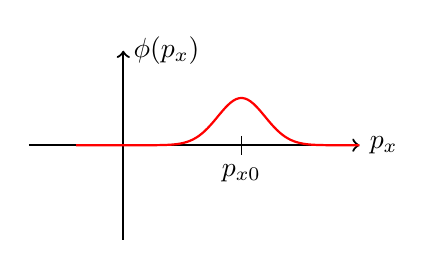
\begin{tikzpicture}[scale=0.6]
\draw[->,thick] (-2,0) -- (5,0) node[right]{$p_x$};
\draw[->,thick] (0,-2) -- (0,2) node[right]{$\phi(p_x)$};
\draw[domain=-1:5,samples=100,thick,red] plot({\x},{exp(-2*(\x-2.5)^2});
\draw (2.5,.2) -- (2.5,-.2)node[below]{$p_{x0}$};
\end{tikzpicture}
\caption[][2cm]{ }
\label{fig:ex211a}
\end{figure}

\sol So we have the initial momentum wavefunction and we insert this into Eq.~(\ref{eq:tdsefreesolint}):
\beq
\psi(x,t) = \sqrt{\frac{\hbar}{2\pi}}  \intii\phi(\hbar k,0) \E{\I(kx-\omega t)}dk
\eeq
We get
\beq
\psi(x,t)=\sqrt{\frac{\hbar}{2\pi}}  \int\displaylimits_{-\infty}^{\infty}\sqrt{\frac{1}{\sigma_p \sqrt{2\pi}}}\E{-\left(\frac{\hbar k - p_{x0}}{2\sigma_p}\right)^2} \E{\I(kx-\omega t)}dk.
\eeq

This is really messy and doesn't simplify easily. However, using our \CAS we run the integral, and find the probability 
\beq
P(x_1,x_2) =\int_{x_1}^{x_2} \psi^{*}(x,t)\psi^{}(x,t)dx.
\eeq 
In the end, the probability of measuring the atom between two positions goes up and down as a function of time, as we expect. We plot this in Figure~\ref{fig:ex211b}
\begin{figure}
\centering
\begin{sagesilent}
x=var('x')
t = var('t')
x_coords = [t for t in srange(-1.0,5.0,.1)]
y_coords = [2.5*(-erf((2*t-3)/sqrt(.5+2*t^2)) + erf((2*t-2)/sqrt(.5+2*t^2))) for t in srange(-1.0,5.0,.1)]
output = ""
for i in range(0,len(x_coords)-1):
    output += r"\draw[red, thick] (%f cm ,%f cm)--(%f cm ,%f cm);"%(x_coords[i],y_coords[i],x_coords[i+1],y_coords[i+1])
\end{sagesilent}

\begin{tikzpicture}
\draw[->,thick] (-1,0) -- (5,0) node[right]{$t$};
\draw[->,thick] (0,-.2) -- (0,2) node[right]{$P(x_1,x_2)$};
\sagestr{output}
\end{tikzpicture}
\caption[][2cm]{ }
\label{fig:ex211b}
\end{figure}

\assess We expect the atom to move through the region at some point, then to move out. So the probability of measuring it in the region makes sense.

\end{example}

\begin{exercise}
Show that the wavefunction from Eq.~(\ref{eq:tdsefreesol}) is a solution to the second-order differential equation (\ref{eq:tdseforfree})
\end{exercise}

\section{Velocity and Momentum}

We now show that our choice for the momentum operator in the position basis, Eq.~(\ref{eq:momentummatrix}) was a good one. We expect that the atom's velocity should be related to is average position:
\beq
v \equiv \frac{d}{dt}\avg{\hat{X}}.
\eeq
We'll expand the average in the position basis:
\bas
v = & \frac{d}{dt}\left(\bra{\Psi}\hat{X}\ket{\Psi}\right) \\
 = & \frac{d}{dt} \int\displaylimits_{-\infty}^{\infty} \psi^*(x,t) x \psi(x,t)dx.
\eas\marginnote[-1cm]{Using \ref{tool:span} and \ref{tool:wavefunction}.}%
But we know that the time derivative of an operator is related to the average of the commutator of the operator with the Hamiltonian, Eq.~(\ref{eq:timeop}):
\beq
\frac{d}{dt}\avg{\hat{X}} = \frac{\I}{\hbar}\avg{\com{\hat{H},\hat{X}}}.
\eeq
We need to do the commutator for the free-space Hamiltonian. This gives us\marginnote{This will be an exercise, too.}
\beq
\com{\frac{\hat{P}_x^2}{2m},\hat{X}} = -\frac{\I\hbar}{m}\hat{P}_x.
\label{ex:fscom}
\eeq
So we get for our velocity
\beq
v = \frac{\avg{\hat{P}_x}}{m}
\eeq
which matches nicely with what we would expect.

\begin{exercise}
Show that the commutator in Eq.~(\ref{ex:fscom}) is correct.
\end{exercise}


\begin{example}
What is the velocity for the atom from Example \ref{ex:gaussatom1}?

\model We again model our atom as having the momentum wavefunction
\beq
\phi(p_x,0) = \sqrt{\frac{1}{\sigma_p \sqrt{2\pi}}}\E{-\left(\frac{p_x - p_{x0}}{2\sigma_p}\right)^2}
\eeq
where $\sigma_p$ is the width of the Gaussian. We'll find the average momentum and use that to get the velocity. It makes sense to work in the momentum basis here.

\vis This is the same picture as before.

\sol We need the average momentum. In terms of the momentum basis
\beq
\avg{\hat{P}_x} =  \int\displaylimits_{-\infty}^{\infty} \phi^*(p_x)p_x\phi(p_x)dp_x = p_{x0}.
\eeq\arnote[-1cm]{Work out the integral on your own.}%
So the velocity is just $p_{x0}/m$.

\assess The units are right and it makes sense given the initial Gaussian momentum wavefunction centered at $p_{x0}$.

\end{example}

\begin{exercise}
\label{ex:firstgauss}
An atom traveling in a line is given an initial position wavefunction
\beq
\psi(x,0) = \frac{1}{(2\pi\sigma_x^2)^{1/4}}\E{-(x-x_0)^2/(4\sigma_x^2)}\E{\I p_0 x/\hbar}.
\eeq
What is the atom's velocity?

\end{exercise}

\begin{exercise}
What if we model an atom traveling in a line with the initial momentum wavefunction
\beq
\phi(p_x,0) = \sqrt{p_{x0}}\delta(p_x - p_{x0});
\eeq
what is the position wavefunction $\psi(x,t)$? Is it normalized? Explain.

\end{exercise}


\chapter{Part \ref{part2} Summary and Test}

In this part we have covered models that describe the time evolution of the quantum state based on the Hamiltonian. We covered states that utilize multiple parameters to describe the quantum system and how those parameters are connected through the uncertainty relationship. We moved to multiple quantum systems and modeled pure states, mixed states and entangled states. We used this to model the measurement process. Finally we moved to continuous parameters describing  quantum states and focused on one-dimensional position and momentum.

It is important to practice using these tools to model experiments. The following set of exercises is a good way to test your understanding of these models. Try to do these without referring to the previous text. If you can do all of them and your solutions agree with those provided on the following pages, then you are in pretty good shape to move forward with the material. If not, you should specifically review the material  you do not have mastery of yet, then retry the test exercises.

\begin{exercise}
 A student is wondering if she can write the momentum wave function of a free particle of mass $m$ in an infinitely long tube as 
%
\begin{equation}
\phi(p_{x}) = \left\{\begin{array}{ll}
                 A\cos(\pi p_{x}/p_{0}), & -p_{0}/2 \leq p_{x} \leq p_{0}/2, \\
                 0 & \mbox{otherwise}
                 \end{array} \right.
\end{equation}
%
 where $p_{0}$  and $A$ are  constants.

\begin{enumerate}

\item  How would you respond to her? (Is this a physically acceptable wave function?)  Explain.

\item   Determine $A$.  What are its units?

\item If you measured  $p_{x}$ of many particles prepared in this state, find the rms deviation $\Delta P_{x}$ of the results.


\end{enumerate}

\end{exercise}


\begin{exercise}
\begin{enumerate}
\item What is the normalized position wavefunction corresponding to the normalized momentum distribution from the previous exercise?

\item  Find the probability that the particle's \underline{position} would be measured within the region $0 \leq x \leq \hbar/p_{0}$.

\item Is the Heisenberg Uncertainty Principle satisfied for this wavefunction? What is $\Delta X \Delta P_x$?

\end{enumerate}


\end{exercise}


\begin{exercise}
A hypothetical quantum system has a Hamiltonian $\hat{H}$ and an observable $\hat{L}$  given by 
%
\beq
 \hat{H} \Rightarrow E_0\left(\begin{array}{ccc}
           3 & 0 & 0 \\
           0 & 2 & 0 \\
           0 & 0 & 1
\end{array}\right)
%
\rmt{ and }
 \hat{L}\Rightarrow \ell_0\left(\begin{array}{ccc}
           0 & \I &1 \\
           -\I & 0 & 0 \\
           1 & 0 & 0 
\end{array}\right),
\eeq
where our basis is the set of energy eigenvectors $\ket{1}$, $\ket{2}$, and $\ket{3}$. The system starts in the state
\beq
\ket{\Psi(0)} = \frac{1}{\sqrt{7}}\ket{1} + \sqrt{\frac{3}{7}}\ket{2} + \I\sqrt{\frac{3}{7}}\ket{3}.
\eeq
\begin{enumerate}
\item  Is $\hat{L}$ conserved?  How can you tell?
\item What is $\ket{\Psi(t)}$?
\item What is $\avg{\hat{L}(t)}$?
\end{enumerate}
\end{exercise}

\begin{exercise}
%density operator + entangled state
Suppose you are given Alice's part of the quantum state
\beq
\ket{\Psi} = \frac{1}{2}\ket{HH} - \sqrt{\frac{3}{8}}\left[\ket{HV} + \ket{VH}\right].
\eeq
\begin{enumerate}
\item What is Alice's reduced density matrix?
\item Is the original state an entangled state or a product state? How can you tell?
\item If Alice measures $\hat{\sigma}_2$ many times with identical copies of her state, what will the average measurement be?
\end{enumerate}

\end{exercise}


Stop here and don't continue reading until you have completed the exercises.
\newpage
\begin{example} 
 A student is wondering if she can write the momentum wave function of a free particle of mass $m$ in an infinitely long tube as 
%
\begin{equation}
\phi(p_{x}) = \left\{\begin{array}{ll}
                 A\cos(\pi p_{x}/p_{0}), & -p_{0}/2 \leq p_{x} \leq p_{0}/2, \\
                 0 & \mbox{otherwise}
                 \end{array} \right.
\end{equation}
%
 where $p_{0}$  and $A$ are  constants.

\begin{enumerate}

\item  This isn't a physically acceptable wavefunction. We plot the wavefunction in Figure ~\ref{fig:351} and see that, although it is continuous, it is not smooth. There aren't real-world situations where the wavefunction will have sharp corners like this.
\begin{figure}
\centering
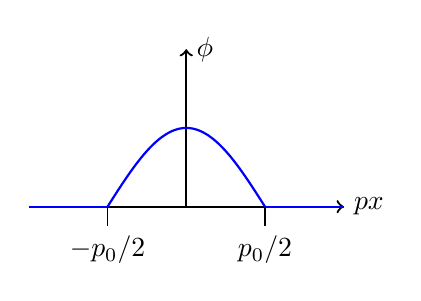
\begin{tikzpicture}
\draw[->,thick] (-2,0) -- (2,0) node[right]{$px$};
\draw[->,thick] (0,0) -- (0,2) node[right]{$\phi$};

\draw[domain=-1:1,samples=100,thick,blue] plot({\x},{cos(\x*90)});
\draw[thick,blue] (-2,0) -- (-1,0);
\draw[thick,blue] (1,0) -- (2,0);
\draw (-1,0) -- (-1,-.25) node[below]{$-p_0/2$};
\draw (1,0) -- (1,-.25) node[below]{$p_0/2$};
\end{tikzpicture}
\caption[][1cm]{ }
\label{fig:351}
\end{figure}


\item  Although the wavefunction is not physical, we still want to work with it and see how it behaves. We need to normalize this:
\beq
1= \intii \phi^{*}(p_x)\phi(p_x)dp_x = \int\displaylimits_{-p_0/2}^{p_0/2}\abs{A}^2\cos^2(\pi p_x/p_0)dp_x = \frac{\abs{A}^2 p_0}{2}.
\eeq
So we have $A = \sqrt{2/p_0}$.

\item We consider a measurement of the momentum $p_{x}$ of many particles prepared in this state, and want the rms deviation $\Delta P_{x}$ of the results. We need two things to calculate this: $\avg{\hat{P}_x}$ and $\avg{\hat{P}^2_x}$. We do both of these:
\beq
\avg{\hat{P}_x} =  \int\displaylimits_{-p_0/2}^{p_0/2}\frac{2}{p_0}p_x\cos^2(\pi p_x/p_0)dp_x = 0
\eeq
and
\beq
\avg{\hat{P}^2_x} =  \int\displaylimits_{-p_0/2}^{p_0/2}\frac{2}{p_0}p^2_x\cos^2(\pi p_x/p_0)dp_x = \frac{p_0^2\left(\pi^2 - 6\right)}{12\pi^2}.
\eeq
The uncertainty in measuring the momentum is then
\beq
\Delta P_x = \sqrt{\avg{\hat{P}^2_x} - \avg{\hat{P}_x}^2} = p_0\sqrt{\frac{\left(\pi^2 - 6\right)}{12\pi^2}}.
\eeq
\end{enumerate}

\end{example}

\begin{example}
\begin{enumerate}
\item We now want the  normalized position wavefunction corresponding to the momentum wavefunction from the previous example. We use the Fourier transform to find this:
\bas
\psi(x) =& \frac{1}{\sqrt{2 \pi \hbar}}\int\displaylimits_{-p_0/2}^{p_0/2}\sqrt{\frac{2}{p_0}}\cos(\pi p_x/p_0)\E{\I p_x x/\hbar}dp_x \\
=&\sqrt{p_0 4\pi\hbar^3}\frac{\cos\left({\frac{p_0 x}{2\hbar}}\right)}{\pi^2\hbar^2 - p_0^2 x^2}.
\eas
We check the normalization of this wavefunction and find
\beq
\intii p_0 4\pi\hbar^3 \frac{\cos^2\left({\frac{p_0 x}{2\hbar}}\right)}{\left(\pi^2\hbar^2 - p_0^2 x^2\right)^2}dx = 1
\eeq
as we need for a normalized wavefunction. The position wavefunction is shown in Figure \ref{fig:352s}.

\begin{marginfigure}
\centering
\begin{tikzpicture}
\draw[->,thick] (-2.5,0) -- (2.5,0) node[right]{$px$};
\draw[->,thick] (0,0) -- (0,2) node[right]{$\psi$};
\begin{sagesilent}
x=var('x')
t = var('t')
x_coords = [t for t in srange(-2.5,2.5,.01)]
y_coords = [4*sqrt(4*3.141)*cos(t*20/2)/(3.141^2-(t*20)^2) for t in srange(-2.5,2.5,.01)]
output352 = ""
for i in range(0,len(x_coords)-1):
    output352 += r"\draw[red, thick] (%f cm ,%f cm)--(%f cm ,%f cm);"%(x_coords[i],y_coords[i],x_coords[i+1],y_coords[i+1])
\end{sagesilent}
\sagestr{output352}

\draw (-1,0) -- (-1,-.25) node[below]{$-20\hbar/p_0$};
\draw (1,0) -- (1,-.25) node[below]{$20\hbar/p_0$};
\end{tikzpicture}
\caption{ }
\label{fig:352s}
\end{marginfigure}

\item  We now want the probability that the particle's position would be measured within the region $0 \leq x \leq \hbar/p_{0}$. We use the probability density to find this:
\bas
P(0 \leq x \leq \hbar/p_{0}) =& \int\displaylimits_{0}^{\hbar/p_0} \psi^*(x)\psi(x)dx \\
=&\int\displaylimits_{0}^{\hbar/p_0}  p_0 4\pi\hbar^3 \frac{\cos^2\left({\frac{p_0 x}{2\hbar}}\right)}{\left(\pi^2\hbar^2 - p_0^2 x^2\right)^2}dx\\
\approx& 0.127.
\eas

\item Finally, we want $\Delta X \Delta P_x$ to check to see if $\Delta X \Delta P_x \geq \hbar/2$. We need $\Delta X$ first.
\beq
\avg{\hat{X}} = \intii p_0 4\pi\hbar^3 \frac{\cos^2\left({\frac{p_0 x}{2\hbar}}\right)}{\left(\pi^2\hbar^2 - p_0^2 x^2\right)^2}x dx = 0
\eeq
\beq
\avg{\hat{X}^2} = \intii p_0 4\pi\hbar^3 \frac{\cos^2\left({\frac{p_0 x}{2\hbar}}\right)}{\left(\pi^2\hbar^2 - p_0^2 x^2\right)^2}x^2 dx = \frac{\pi^2 \hbar^2}{p_0^2}
\eeq
So $\Delta X = \pi\hbar/p_0$. Therefore,
\beq
\Delta X \Delta P_x = \sqrt{\frac{\pi^2-6}{12}}\hbar \approx 0.57\hbar
\eeq
so we have satisfied the Heisenberg Uncertainty Principle with this state.
\end{enumerate}
\end{example}

\begin{example}
We have a hypothetical quantum system with a Hamiltonian $\hat{H}$ and an observable $\hat{L}$  which are given by 
%
\beq
 \hat{H} \Rightarrow E_0\left(\begin{array}{ccc}
           3 & 0 & 0 \\
           0 & 2 & 0 \\
           0 & 0 & 1
\end{array}\right) \rmt{ and }
%
 \hat{L}\Rightarrow \ell_0\left(\begin{array}{ccc}
           0 & \I &1 \\
           -\I & 0 & 0 \\
           1 & 0 & 0 
\end{array}\right),
\eeq
where our basis is the set of energy eigenvectors $\ket{1}$, $\ket{2}$, and $\ket{3}$. The system starts in the state
\beq
\ket{\Psi(0)} = \frac{1}{\sqrt{7}}\ket{1} + \sqrt{\frac{3}{7}}\ket{2} + \I\sqrt{\frac{3}{7}}\ket{3}.
\eeq
\begin{enumerate}
\item  We first want to know if $\hat{L}$ is conserved? If $\com{\hat{H},\hat{L}}=0$, then the average measurement of $\hat{L}$ doesn't change and $\hat{L}$ is conserved. So we check the commutation relationship:
\beq
\com{\hat{H},\hat{L}} = \hat{H}\hat{L} - \hat{L}\hat{H} = E_0 \ell_0 \left(\begin{array}{ccc}
           0 & \I & 2 \\
           \I & 0 & 0 \\
           -2 & 0 & 0 
\end{array}\right)\neq 0
\eeq
so this is not a conserved quantity (or $d\avg{\hat{L}}/dt \neq 0$).

\item We want to know what the time evolution is, so we first find $\ket{\Psi(t)}$. Using the technique \ref{tactis:TISE}, we first need to know what the energies are for the three eigenstates. We notice that $\hat{H}$ is diagonal, so 
\bas
\hat{H}\ket{1} = & 3E_0\ket{1}\\
\hat{H}\ket{2} = & 2E_0\ket{2}\\
\hat{H}\ket{3} = & E_0\ket{3}.
\eas
Therefore, the time-dependent state is
\beq
\ket{\Psi(t)} = \frac{1}{\sqrt{7}}\E{-\I 3E_0 t/\hbar}\ket{1} + \sqrt{\frac{3}{7}}\E{-\I 2E_0 t/\hbar}\ket{2} + \I\sqrt{\frac{3}{7}}\E{-\I E_0 t/\hbar}\ket{3}.
\eeq

\item Finally, we find $\avg{\hat{L}(t)}$:
\bas
\avg{\hat{L}(t)} =& \bra{\Psi(t)}\hat{L}\ket{\Psi(t)}\\
=& -\frac{2\ell_0\sqrt 3}{7}\left[\sin\left(\frac{E_0 t}{\hbar}\right)+\sin\left(\frac{2 E_0 t}{\hbar}\right)\right]
\eas
\end{enumerate}
\end{example}

\begin{example}
We are given Alice's part of the quantum state
\beq
\ket{\Psi} = \frac{1}{2}\ket{HH} - \sqrt{\frac{3}{8}}\left[\ket{HV} + \ket{VH}\right].
\eeq
\begin{enumerate}
\item We first want Alice's reduced density matrix. Using the reduced density matrix definition from Eq.~(\ref{eq:reduceddensitymatrixcomp}).
\bas
\rho_{HH} = & \alpha^{}_{HH}\alpha^*_{HH} + \alpha^{}_{HV}\alpha^*_{HV} = \frac{5}{8} \\
\rho_{HV} = & \alpha^{}_{HH}\alpha^*_{VH} + \alpha^{}_{HV}\alpha^*_{VV} = -\sqrt{\frac{3}{32}} \\
\rho_{VH} = & \alpha^{}_{VH}\alpha^*_{HH} + \alpha^{}_{VV}\alpha^*_{HV} = -\sqrt{\frac{3}{32}} \\
\rho_{VV} = & \alpha^{}_{VH}\alpha^*_{VH} + \alpha^{}_{VV}\alpha^*_{VV} = \frac{3}{8}.
\eas
So we have the reduced density matrix
\beq
\hat{\rho}_\rmt{Alice} = \begin{pmatrix}\frac{5}{8}&-\sqrt{\frac{3}{32}}\\-\sqrt{\frac{3}{32}}&\frac{3}{8}\end{pmatrix}.
\eeq
\item This doesn't look like a maximally entangled density matrix, but it also doesn't look like a product state density matrix. We see that we can't factorize the original state, so it must be entangled.
\item We also want the average measurement of $\hat{\sigma}_2$ for many measurements using the initial identical state. However, since Alice only has access to her piece of the state, she only measures using her reduced density operator. The average measurement is then
\beq
\avg{\hat{\sigma}_2} = \Tr\left(\hat{\rho}\hat{\sigma}_2\right) \Meq \Tr\begin{pmatrix}\frac{5}{8}&-\sqrt{\frac{3}{32}}\\-\sqrt{\frac{3}{32}}&\frac{3}{8}\end{pmatrix}\symatrix  = 0.
\eeq
We might have expected this result, since Alice's state is in the $V-H$ basis and not in the $C_R-C_L$ basis.
\end{enumerate}
\end{example}




%sagemathcloud={"latex_command":""}